\documentclass[twoside,10pt]{article}

\usepackage[T1]{fontenc}
\usepackage{lmodern}
\usepackage{amsmath,amsthm,amssymb,amsfonts}
\usepackage{mathtools}
\usepackage[small,labelfont=bf,labelsep=period]{caption}
\usepackage[
  letterpaper,
  total={5.5in,8in},
  vmarginratio=1:1,
  hmarginratio=1:1,
  headsep=21pt
]{geometry}
\usepackage{xcolor}
\usepackage{tikz}
\usepackage[
  breaklinks=false,
  linktocpage=true
]{hyperref}
\hypersetup{
  colorlinks=true,
  linkcolor={purple},
  urlcolor={purple},
  citecolor={blue!80!black},
  pdfauthor={Leslie P. Polzer},
  pdftitle={Zamolodchikov's Large-Weight Limit for Sphere Four-Point Virasoro Blocks},
  pdfsubject={Large-dimension asymptotics, fixed-charge confluence, and sharp Jantzen pole orders for sphere four-point Virasoro conformal blocks},
  pdfkeywords={Virasoro algebra, conformal blocks, sphere four-point block, Zamolodchikov recursion, minimal models, Jantzen filtration, Ising model}
}

\medmuskip=4mu
\thickmuskip=8mu
\setlength{\emergencystretch}{2em}

\numberwithin{equation}{section}

\newtheoremstyle{slbody}
  {8pt}
  {8pt}
  {\normalfont\slshape}
  {}
  {\bfseries}
  {.}
  {0.5em}
  {\thmname{#1}\thmnumber{ #2}%
   \thmnote{ {\normalfont\itshape(\ignorespaces#3\unskip)}}}
\theoremstyle{slbody}
\newtheorem{theorem}{Theorem}[section]
\newtheorem{proposition}[theorem]{Proposition}
\newtheorem{lemma}[theorem]{Lemma}
\newtheorem{corollary}[theorem]{Corollary}
\theoremstyle{definition}
\newtheorem{definition}[theorem]{Definition}
\theoremstyle{remark}
\newtheorem{remark}[theorem]{Remark}
\newtheorem*{remark*}{Remark}
\newtheorem*{example*}{Example}

\renewcommand{\qedsymbol}{$\blacksquare$}

\newcommand{\Vir}{\operatorname{Vir}}
\newcommand{\CT}{\operatorname{CT}}
\newcommand{\ord}{\operatorname{ord}}
\newcommand{\Tr}{\operatorname{Tr}}
\newcommand{\Res}{\operatorname{Res}}

\title{Zamolodchikov's large-weight limit for sphere four-point\\
Virasoro blocks}
\author{Leslie P. Polzer}
\newcommand{\authoraffiliation}{Independent Researcher}
\newcommand{\authoremail}{polzer@fastmail.com}
\date{November 25, 2026}

\makeatletter
\renewcommand{\section}{%
  \@startsection{section}{1}{\z@}%
    {-3.5ex \@plus -1ex \@minus -.2ex}%
    {2.3ex \@plus .2ex}%
    {\normalfont\large\bfseries}}
\renewcommand{\@seccntformat}[1]{%
  \csname the#1\endcsname.\enspace}

\newcommand{\shorttitle}{LARGE-WEIGHT LIMIT OF SPHERE VIRASORO BLOCKS}
\newcommand{\shortauthors}{LESLIE P. POLZER}
\newcommand{\ps@bookheader}{%
  \renewcommand\@oddfoot{\hfil}%
  \renewcommand\@evenfoot{\hfil}%
  \renewcommand\@oddhead{%
    \ifnum\value{page}>1
      {\small\hfil\shortauthors}\hfil\thepage
    \else
      \hfil
    \fi}%
  \renewcommand\@evenhead{%
    \thepage\hfil\small\shorttitle\hfil}}
\pagestyle{bookheader}

\renewcommand{\maketitle}{%
  \begin{center}
    {\large\bfseries\@title}\\
    \vskip36pt
    \ifx\@author\@empty
      \mbox{}\par
    \else
      {\scshape\@author}\par
      \medskip
      {\small\authoraffiliation}\par
      \smallskip
      {\small\texttt{\authoremail}}\par
      \smallskip
      {\small\@date}\par
    \fi
    \vskip36pt
  \end{center}}
\makeatother

\renewenvironment{abstract}
  {\quotation\noindent\small{\bfseries\abstractname.\enspace}}
  {\endquotation}

\begin{document}
\maketitle

\begin{abstract}
We prove Zamolodchikov's large-internal-weight limit \(H_N\to\delta_{N,0}\)
for the elliptic coefficients of the sphere four-point Virasoro block, for
each \(N\geq0\) and all complex central charges and external weights.  The
limit fixes the polynomial part in Zamolodchikov's recursion in the internal
weight.  The proof writes the block in a Feigin--Fuchs oscillator
realization, evaluates the leading Gaussian term at an explicit saddle point,
computes its determinant from a symmetric kernel on the elliptic curve
\(y^2=x(x-1)(x-z)\), and obtains the central-charge exponent from the
diagonal Virasoro action on two \(c=1\) Fock modules.
\end{abstract}

\section{Introduction}\label{sec:intro}

To solve the crossing equations of a two-dimensional conformal field theory
numerically, one has to compute Virasoro conformal blocks to high
order~\cite[\S4.3]{Ribault2026}.  The \(s\)-channel sphere four-point block is
\[
 \mathcal F(c,\Delta,\Delta_1,\Delta_2,\Delta_3,\Delta_4;z)
 =z^{\Delta-\Delta_1-\Delta_2}\sum_{N=0}^\infty\mathcal B_N(c,\Delta,\Delta_i)z^N.
\]
Each \(\mathcal B_N\) pairs two three-point vectors through the inverse
level-\(N\) Shapovalov matrix of the Verma module \(M(c,\Delta)\), a matrix
whose size is the number of partitions of \(N\).  Computing blocks from this
definition is inefficient, and Zamolodchikov's recursions avoid the matrix
inversion~\cite[\S4.3]{Ribault2026}.  He gave a central-charge recursion at
fixed internal weight~\cite[(8)]{Zamolodchikov1984} and a recursion in the
internal weight, which is the one studied here~\cite{Zamolodchikov1987}.  For
generic \(c=c(b)=1+6(b+b^{-1})^2\) he wrote \(\mathcal F=\Phi H\) in the nome
\(q(z)\)~\cite[(5)--(6)]{Zamolodchikov1987}, where \(\Phi\) is an explicit
elliptic prefactor.  Each coefficient \(H_N\) of
\(H=\sum_{N\geq0}H_N(c,\Delta,\Delta_i)(16q)^N\) is a rational function of
\(\Delta\) with at most simple poles, at the Kac weights \(h_{r,s}(b)\) with
\(rs\leq N\)~\cite[\S3]{Zamolodchikov1987}.\footnote{The poles are (16)--(17) of~\cite{Zamolodchikov1987}; the residues are given in the recursion that follows (17).}
Its residue at \(h_{r,s}(b)\) is an explicit factor times \(H_{N-rs}\) at the
shifted weight \(h_{r,s}(b)+rs\).  A rational function is the sum of
its principal parts and a polynomial, so the lower coefficients determine
\(H_N\) once its polynomial part is known.  Zamolodchikov fixed the polynomial
part by the large-weight limit \(H_N\to\delta_{N,0}\) as \(\Delta\to\infty\).
Numerical bootstrap computations truncate the resulting
series~\cite[\S4.4.2]{Ribault2026}.

Ribault calls the large-weight limit the most important piece of the
derivation of the recursion and notes that a complete derivation appears to
be missing~\cite[\S4.3.4]{Ribault2026}; Zamolodchikov's argument uses
semiclassical monodromy, a degree argument and a comparison at
\(c=1\)~\cite{Zamolodchikov1987}.  Theorem~\ref{thm:large-delta} proves the
limit: for every \(N\geq0\) and every
\((c,\Delta_1,\dots,\Delta_4)\in\mathbb C^5\),
\[
 \lim_{\Delta\to\infty}H_N(c,\Delta,\Delta_1,\Delta_2,\Delta_3,\Delta_4)=\delta_{N,0}.
\]
Together with the residues at the Kac weights, this gives Zamolodchikov's
recursion; the companion paper writes out the residues and the
recursion~\cite[Proposition~12.4]{PolzerColliding2026}
and treats rational \(b^2\), where Kac weights coincide and the recursion
breaks down~\cite[\S4.3.3]{Ribault2026}.

In one case the prefactor is the whole block: at \(c=1\) with
\(\Delta_1=\dots=\Delta_4=\frac1{16}\), the chiral weight of the spin (twist)
fields of the critical Ashkin--Teller model, \(H=1\) at every intermediate
weight \(\Delta\) at which \(M(1,\Delta)\) is
irreducible~\cite[(2.28)]{Zamolodchikov1986} (see the remark at the end of
Section~\ref{sec:asymp}).  As rational functions of \(\Delta\), the
coefficients \(H_N\) with \(N\geq1\) then vanish identically.
Theorem~\ref{thm:large-delta} says that for all parameters \(H\) tends to
\(1\) as \(\Delta\to\infty\), coefficient by coefficient in \(q\).  Ribault
reviews a geometric reading of the factors of \(\Phi\) through the conformal
map from the four-punctured sphere to a pillow, the quotient by
\(u\mapsto-u\) of the torus \(y^2=x(x-1)(x-z)\) with coordinate \(u\)
proportional to \(\int^x dx'/y\)~\cite[\S4.3.4]{Ribault2026}.\footnote{Equations (4.42)--(4.44) of~\cite{Ribault2026}.}  There the factor
\(q^\Delta\) is time evolution along the pillow, the factors that depend on
the \(\Delta_i\) come from transforming the four fields, which sit at its
corners, and the factor that depends on \(c\) comes from the Weyl anomaly.
Our proof obtains these factors in the Fock space, and the Gaussian
determinant from a kernel on the same torus.

The proof is a saddle-point computation.  Take
\(c=1+24\eta^2>1\), real external weights and \(\Delta=\omega^2+\eta^2\) with
\(\omega>0\).  The Feigin--Fuchs realization identifies the Verma module with a
Fock space of oscillators \(u_m\), and the block pairs two solutions \(F\) of
the Ward equations there.  After the rescaling
\(u_m=\omega\sigma_m\), \(F=\exp(\omega^2S)\) with \(S\) a series in
\(\omega^{-1}\), so \(\omega^2\) plays the
role of \(1/\hbar\), and as \(\omega\to\infty\) the coefficientwise Gaussian
calculation of the pairing is centered at a saddle point
(Proposition~\ref{prop:gaussian-limit}).  Each factor of
Zamolodchikov's prefactor then has its own source, displayed at the start of
Section~\ref{sec:asymp}: the value at the saddle point
(Lemma~\ref{lem:saddle}), the Gaussian determinant
(Lemma~\ref{lem:bergman-det}), and the first corrections, which are linear in
the external weights (Lemma~\ref{lem:ext-exponents}) and in
\(\eta^2=(c-1)/24\) (Lemma~\ref{lem:central-charge}).  The Gaussian
calculation defines the last correction only through the Ward hierarchy.
Lemma~\ref{lem:central-charge} evaluates it by a comparison at \(c=2\): the
product of two Gaussian Ward solutions on two \(c=1\) Fock modules solves the
\(c=2\) Ward equations exactly, and decomposing the tensor product into
\(c=2\) Verma modules gives an identity that determines the exponent.
Lemma~\ref{lem:fock-verma}(iii) extends the limit to complex parameters.

Be\c{s}ken--Datta--Kraus obtain the leading exponential \((16q)^\Delta\)
and set aside the determinant and Jacobian prefactors
\cite[\S4.3]{BeskenDattaKraus2019}.\footnote{Equations (4.23)--(4.25) of~\cite{BeskenDattaKraus2019}.}  Artemev and Khromov use
WKB for the classical BPZ equation to obtain large-intermediate-dimension
asymptotics of comb-channel blocks~\cite{ArtemevKhromov2026}.  Ghosal, R\'emy,
Sun and Sun prove that the normalized sphere block is analytic in \(z\) for
\(|z|<1\) and meromorphic in \(\Delta\), for \(c>25\) and their stated range of
external momenta \cite[Theorem~1.2]{GhosalRemySunSun2022}; their theorem gives
no large-\(\Delta\) limit.

Section~\ref{sec:setup} fixes definitions and normalizations, and
Section~\ref{sec:asymp} proves the limit.  Appendix~\ref{app:gaussian}
contains the finite-sum bookkeeping for the Gaussian calculation of
Proposition~\ref{prop:gaussian-limit}.

\section{Definitions and normalizations}\label{sec:setup}

Let \(\Vir=\bigoplus_{n\in\mathbb Z}\mathbb C L_n\oplus\mathbb C C\) be the
Virasoro algebra with
\([L_m,L_n]=(m-n)L_{m+n}+\frac{m^3-m}{12}\delta_{m+n,0}C\).  For
\(c,\Delta\in\mathbb C\), let \(M(c,\Delta)\) be the Verma module with
highest-weight vector \(v_\Delta\), so that \(L_0v_\Delta=\Delta v_\Delta\)
and \(L_n v_\Delta=0\) for \(n>0\).  For a partition
\(Y=(y_1\geq\dots\geq y_r\geq1)\) of \(N\) write
\(L_{-Y}=L_{-y_1}\cdots L_{-y_r}\); the vectors \(L_{-Y}v_\Delta\) with
\(|Y|=N\) form the PBW basis of level \(N\), of dimension the number \(p(N)\) of
partitions of \(N\).  We write \(\Vir_-\) for the span of the \(L_{-n}\),
\(n\geq1\).  Let
\(G_N(c,\Delta)_{Y,Z}=\langle L_{-Y}v_\Delta,L_{-Z}v_\Delta\rangle\) be the
Shapovalov Gram matrix for the contravariant bilinear form normalized by
\(\langle v_\Delta,v_\Delta\rangle=1\) and \((L_n)^\dagger=L_{-n}\).

\begin{definition}[Three-point pairing and sphere block]\label{def:sphere-block}
For indeterminate weights \(\Delta,\Delta_a,\Delta_b\) and a partition
\(Y=(y_1\geq\dots\geq y_r\geq1)\), define the three-point polynomial
\begin{equation}\label{eq:gamma-Y}
 \Gamma_Y(\Delta;\Delta_a,\Delta_b)
 :=\prod_{j=1}^r\Bigl(\Delta+\sum_{i=j+1}^r y_i+y_j\Delta_b-\Delta_a\Bigr)
 \in\mathbb Z[\Delta,\Delta_a,\Delta_b],
\end{equation}
with \(\Gamma_\emptyset=1\).  Let \(\langle u\mid V_{\Delta_b}(1)\mid\Delta_a\rangle\)
denote the unique linear functional on \(M(c,\Delta)\) with
\(\langle v_\Delta\mid V_{\Delta_b}(1)\mid\Delta_a\rangle=1\) and
\(\langle L_{-n}u\mid V_{\Delta_b}(1)\mid\Delta_a\rangle
=(h(u)+n\Delta_b-\Delta_a)\langle u\mid V_{\Delta_b}(1)\mid\Delta_a\rangle\) for
homogeneous \(u\) of \(L_0\)-weight \(h(u)\) and \(n\geq1\).  Induction on
\(r\) gives \(\langle L_{-Y}v_\Delta\mid V_{\Delta_b}(1)\mid\Delta_a\rangle
=\Gamma_Y(\Delta;\Delta_a,\Delta_b)\).

The \(s\)-channel Verma sphere four-point block is
\[
 \mathcal F(c,\Delta,\Delta_i;z)
 =z^{\Delta-\Delta_1-\Delta_2}\mathcal B(c,\Delta,\Delta_i;z),
 \qquad
 \mathcal B(c,\Delta,\Delta_i;z)
 =\sum_{N=0}^\infty\mathcal B_N(c,\Delta,\Delta_i)\,z^N,
\]
with \(\mathcal B_0=1\) and, for \(N\geq1\),
\begin{multline}\label{eq:B-def}
 \mathcal B_N(c,\Delta,\Delta_i)
 :=\sum_{|Y|=|Z|=N}\Gamma_Y(\Delta;\Delta_4,\Delta_3)\,
   \bigl(G_N(c,\Delta)^{-1}\bigr)_{Y,Z}\,\Gamma_Z(\Delta;\Delta_1,\Delta_2)\\
 \in\mathbb Q(c,\Delta)[\Delta_1,\Delta_2,\Delta_3,\Delta_4].
\end{multline}
\end{definition}

The order in~\eqref{eq:B-def} places the external primaries of weights
\((\Delta_4,\Delta_3,\Delta_2,\Delta_1)\) at \((\infty,1,z,0)\), so \(\mathcal B_1=(\Delta+\Delta_3-\Delta_4)(\Delta+\Delta_2-\Delta_1)/(2\Delta)\).

\begin{definition}[Elliptic nome and Zamolodchikov \(H\)-series]\label{def:H-series}
Define the Jacobi theta series
\[
 \theta_3(q)=\sum_{n\in\mathbb Z}q^{n^2},\qquad
 \theta_4(q)=\sum_{n\in\mathbb Z}(-1)^n q^{n^2},\qquad
 \theta_2(q)=\sum_{n\in\mathbb Z}q^{(n+1/2)^2}.
\]
The cross-ratio \(z(q):=\theta_2(q)^4/\theta_3(q)^4\) lies in
\(16q(1+q\mathbb Z[[q]])\), and its compositional inverse \(q(z)\) lies in
\(\frac{z}{16}(1+z\mathbb Q[[z]])\).  The series \(q(z)\) is the elliptic nome
\(\exp(-\pi K(1-z)/K(z))\), where
\(K(z)=\frac\pi2{}_2F_1(\tfrac12,\tfrac12;1;z)\).  The theta series and
\(z(q)\) satisfy the classical Jacobi
identities~\cite[\S\S21.2--21.61, 22.3--22.302]{WhittakerWatson1927}:
\begin{gather}
 1-z(q)=\frac{\theta_4(q)^4}{\theta_3(q)^4},\qquad
 {}_2F_1\!\left(\tfrac12,\tfrac12;1;z(q)\right)=\theta_3(q)^2,
 \label{eq:jacobi-1}\\
 z\frac{d}{dz}\log\frac{16q(z)}{z}=\frac{1}{(1-z)\theta_3(q(z))^4}-1,\qquad
 \theta_2(q)\theta_3(q)\theta_4(q)=2q^{1/4}\prod_{m=1}^\infty(1-q^{2m})^3,
 \label{eq:jacobi-2}\\
 16q\prod_{m=1}^\infty(1-q^{2m})^{12}=z(q)(1-z(q))\theta_3(q)^{12}.
 \label{eq:jacobi-3}
\end{gather}
Define Zamolodchikov's prefactor~\cite[\S3, the formula after (18)]{Zamolodchikov1987}
\begin{multline}\label{eq:Phi-def}
 \Phi(c,\Delta,\Delta_i;q)
 :=(16q)^{\Delta-\frac{c-1}{24}}\,
   z(q)^{\frac{c-1}{24}-\Delta_1-\Delta_2}\,
   \bigl(1-z(q)\bigr)^{\frac{c-1}{24}-\Delta_2-\Delta_3}\\
   \times\theta_3(q)^{\frac{c-1}{2}-4(\Delta_1+\Delta_2+\Delta_3+\Delta_4)},
\end{multline}
and the elliptic \(H\)-series
\(H(c,\Delta,\Delta_i;q)=\sum_{N=0}^\infty H_N(c,\Delta,\Delta_i)(16q)^N\)
(\(H_0=1\)) by
\begin{equation}\label{eq:H-def}
 H(c,\Delta,\Delta_i;q)
 :=\widetilde\Phi(c,\Delta,\Delta_i;q)^{-1}
   \sum_{m=0}^\infty\mathcal B_m(c,\Delta,\Delta_i)\,z(q)^m,
\end{equation}
where
\begin{align*}
 \widetilde\Phi(c,\Delta,\Delta_i;q)
 &:=z(q)^{-\Delta+\Delta_1+\Delta_2}\Phi(c,\Delta,\Delta_i;q)\\
 &=\Bigl(\frac{16q}{z(q)}\Bigr)^{\Delta-\frac{c-1}{24}}
  \bigl(1-z(q)\bigr)^{\frac{c-1}{24}-\Delta_2-\Delta_3}
  \theta_3(q)^{\frac{c-1}{2}-4\sum_{j=1}^4\Delta_j}
\end{align*}
lies in \(1+q\mathbb Q[c,\Delta,\Delta_1,\dots,\Delta_4][[q]]\).  Thus
\(\mathcal B=\widetilde\Phi H\) and \(\mathcal F=\Phi H\): the prefactor
\(\Phi\) relates \(H\) to the block, and \(\widetilde\Phi\) relates it to the
cross-ratio series.
\end{definition}

\section{Large-\texorpdfstring{\(\Delta\)}{Delta} asymptotics of the elliptic \texorpdfstring{\(H\)}{H}-series}\label{sec:asymp}

\begin{theorem}[Large-\(\Delta\) decay of \(H_N\)]\label{thm:large-delta}
For every \(N\geq0\) and every \((c,\Delta_1,\Delta_2,\Delta_3,\Delta_4)\in\mathbb C^5\),
\[
 \lim_{\Delta\to\infty}H_N(c,\Delta,\Delta_1,\Delta_2,\Delta_3,\Delta_4)=\delta_{N,0}.
\]
Equivalently, writing \(H_N(c,\Delta,\Delta_i)=P_N(c,\Delta,\Delta_i)/\det G_N(c,\Delta)\)
over the common denominator \(\det G_N(c,\Delta)\) with polynomial numerator
\(P_N\in\mathbb Q[c,\Delta,\Delta_1,\dots,\Delta_4]\), one has
\(\deg_\Delta P_N<\deg_\Delta\det G_N(c,\Delta)\) for every \(N\geq1\).
\end{theorem}

Since \(\mathcal B=\widetilde\Phi H\), the theorem says that
\((16q/z)^{-\Delta}\mathcal B\) tends to \((16q/z)^{-\Delta}\widetilde\Phi\),
which does not depend on \(\Delta\).  The proof obtains this limit as a product
of four factors.  With \(z=z(q)\) and \(\theta_4^4=(1-z)\theta_3^4\),
\[
 \widetilde\Phi
 =\Bigl(\frac{16q}{z}\Bigr)^{\Delta-\frac{c-1}{24}}
  \cdot(1-z)^{-\frac18}\theta_3^{-1}
  \cdot\theta_3^{-4(\Delta_1+\Delta_4-\frac18)}\theta_4^{-4(\Delta_2+\Delta_3-\frac18)}
  \cdot\bigl((1-z)\theta_3^{12}\bigr)^{\frac{c-1}{24}}.
\]
In the order written, the factors are the value at the saddle point
(Lemma~\ref{lem:saddle}), the Gaussian determinant
(Lemma~\ref{lem:bergman-det}), the terms linear in the external weights
(Lemma~\ref{lem:ext-exponents}) and the term linear in
\(\eta^2=(c-1)/24\) (Lemma~\ref{lem:central-charge}).  The proof of the
theorem at the end of the section multiplies them.

\subsection{Fock--Verma equivalence and the \texorpdfstring{\(\omega^{-1}\)}{1/omega}-expansion}

Parameterize \(c=1+24\eta^2\) and \(\Delta=\omega^2+\eta^2\) with
\(\eta,\omega\in\mathbb R_{>0}\).  The polynomial Fock space
\(\mathcal F_{\eta,\omega}=\mathbb C[u_1,u_2,\dots]\) is graded by
\(\deg u_m=m\).  Index the monomials \(u^\alpha=\prod_m u_m^{\alpha_m}\) by
\(\alpha=(\alpha_1,\alpha_2,\dots)\).  For polynomials
\(A(\bar u)=\sum_\alpha A_\alpha\bar u^\alpha\) and
\(B(u)=\sum_\alpha B_\alpha u^\alpha\) in two sets of variables, define the
bilinear pairing
\begin{equation}\label{eq:fock-ip}
 \langle A(\bar u),B(u)\rangle
 :=\sum_{\alpha}A_\alpha\,B_\alpha\prod_{m\geq1}\frac{\alpha_m!}{(2m)^{\alpha_m}}.
\end{equation}
For \(f\in\mathcal F_{\eta,\omega}\), let \(\bar f(\bar u)\) have the complex
conjugate coefficients of \(f\); then \(\langle\bar f,g\rangle\) is a
positive-definite Hermitian inner product on \(\mathcal F_{\eta,\omega}\).
The Feigin--Fuchs differential operators~\cite[\S2.1, (2.2) and (2.5)--(2.6)]{BeskenDattaKraus2019}
\begin{equation}\label{eq:ff-ops}
 \begin{aligned}
  l_0&=\sum_{n=1}^\infty n u_n\partial_{u_n}+\omega^2+\eta^2,\\
  l_k&=\sum_{n=1}^\infty n u_n\partial_{u_{n+k}}
       -\frac14\sum_{n=1}^{k-1}\partial_{u_n}\partial_{u_{k-n}}
       +(\eta k+i\omega)\partial_{u_k}\qquad(k\geq1),\\
  l_{-k}&=\sum_{n=1}^\infty(n+k)u_{n+k}\partial_{u_n}
       -\sum_{n=1}^{k-1}n(k-n)u_nu_{k-n}
       +2k(\eta k-i\omega)u_k\qquad(k\geq1)
 \end{aligned}
\end{equation}
form a Virasoro representation of central charge \(c=1+24\eta^2\), and
\(l_k^\dagger=l_{-k}\) under~\eqref{eq:fock-ip} for real \(\eta,\omega\).

\begin{lemma}[Fock--Verma equivalence and reduction to real parameters]\label{lem:fock-verma}
Fix \(\eta>0\), \(\Delta_1,\dots,\Delta_4\in\mathbb R\), and \(N\geq0\).
\begin{enumerate}\setlength{\itemsep}{1pt}\setlength{\topsep}{3pt}
\item[(i)] For every \(\omega>0\), the Verma module
  \(M(1+24\eta^2,\omega^2+\eta^2)\) is irreducible and isometric to
  \(\mathcal F_{\eta,\omega}\) via \(L_{-Y}v_\Delta\mapsto l_{-Y}1\).
\item[(ii)] The Ward equations \(l_k F=(l_0+k\Delta_2-\Delta_1)F\), for all
  \(k\geq1\), have a unique formal solution
  \(F(u;\omega)=\sum_{m=0}^\infty F_m(u;\omega)\) with \(F_m\) homogeneous
  of level \(m\) and \(F_0=1\).  Let \(\widetilde F(\bar u;\omega)\) be
  obtained from \(F(u;\omega)\) by sending \(u_m\mapsto\bar u_m\),
  \(i\mapsto-i\) and \((\Delta_1,\Delta_2)\mapsto(\Delta_4,\Delta_3)\).  Then
  \(\mathcal B_N(1+24\eta^2,\omega^2+\eta^2,\Delta_i)
  =\langle\widetilde F_N(\bar u;\omega),F_N(u;\omega)\rangle\) for the
  bilinear pairing~\eqref{eq:fock-ip}; the coefficients of
  \(\widetilde F_N\) are not conjugated.
\item[(iii)] If \(\lim_{\omega\to+\infty}H_N(1+24\eta^2,\omega^2+\eta^2,\Delta_i)=\delta_{N,0}\)
  for all \(\eta>0\) and \((\Delta_1,\dots,\Delta_4)\in\mathbb R^4\), then
  Theorem~\ref{thm:large-delta} holds for all
  \((c,\Delta_1,\dots,\Delta_4)\in\mathbb C^5\).
\end{enumerate}
\end{lemma}

\begin{proof}
(i) Write \(c=1+6Q^2\) with \(Q=b+b^{-1}=2\eta>0\).  If \(c\geq25\) then
\(b>0\), so every Kac weight
\(h_{r,s}=\frac14(Q^2-(rb+sb^{-1})^2)\leq0<\omega^2+\eta^2\).  If
\(1<c<25\) then \(b=e^{i\theta}\) with \(\theta\in(0,\pi/2)\); then
\(h_{r,r}=\frac14(1-r^2)Q^2\leq0<\Delta\), while for \(r\neq s\) one has
\(\operatorname{Im}((rb+sb^{-1})^2)=(r^2-s^2)\sin(2\theta)\neq0\) so
\(h_{r,s}\notin\mathbb R\).  By the Kac determinant
formula~\cite[Theorem~4.2]{IoharaKoga2011}, \(\det G_N(c,\Delta)\) vanishes
only at the weights \(h_{r,s}\) with \(rs\leq N\), so
\(\det G_N(c,\Delta)\neq0\) for all \(N\geq0\).  Hence \(M(c,\Delta)\) is
irreducible and unitary, and the
intertwiner \(L_{-Y}v_\Delta\mapsto l_{-Y}1\) is a unitary isomorphism
because \(\dim\mathcal F_{\eta,\omega,N}=p(N)=\dim M(c,\Delta)_N\).

(ii) The level-\(N\) vector \(w_N^{(1,2)}\in M(c,\Delta)_N\) uniquely
characterized by \(\langle L_{-Y}v_\Delta,w_N^{(1,2)}\rangle
=\Gamma_Y(\Delta;\Delta_1,\Delta_2)\) satisfies
\(\langle L_{-Z}v_\Delta,L_kw_N^{(1,2)}\rangle
=(N-k+\Delta+k\Delta_2-\Delta_1)\Gamma_Z(\Delta;\Delta_1,\Delta_2)\), hence
\(L_k w_N^{(1,2)}=(N-k+\Delta+k\Delta_2-\Delta_1)w_{N-k}^{(1,2)}\) for all
\(k\geq1\).  Since \(M(c,\Delta)\) is irreducible, \(F_N\) is the unique
solution to the Ward equations with \(F_0=1\) and equals the image of
\(w_N^{(1,2)}\) in \(\mathcal F_{\eta,\omega}\).  Because the parameters are
real, \(\mathcal B_N=\langle w_N^{(4,3)},w_N^{(1,2)}\rangle\) equals the
stated Fock pairing.

(iii) By the Kac determinant formula~\cite[Theorem~4.2, (4.16) and
(4.21)]{IoharaKoga2011}, \(\det G_m\mid\det G_N\) for
\(m\leq N\).  Since \(\widetilde\Phi^{-1}\) has polynomial coefficients in
\((c,\Delta,\Delta_i)\), it follows that
\(H_N(c,\Delta,\Delta_i)=P_N(c,\Delta,\Delta_i)/\det G_N(c,\Delta)\) with
\(P_N\in\mathbb Q[c,\Delta,\Delta_1,\dots,\Delta_4]\).  As
\(\Delta\to\infty\), \(\det G_N=K_N\Delta^{d_N}+O(\Delta^{d_N-1})\) with a
constant \(K_N>0\).  For
\(N\geq1\), vanishing of \(\lim_{\Delta\to+\infty}H_N\) on the
Zariski-dense real open set \(\{c>1,\ \Delta_i\in\mathbb R\}\) forces every
coefficient of \(\Delta^d\) (\(d\geq d_N\)) in \(P_N\) to vanish
identically as a polynomial in \((c,\Delta_1,\dots,\Delta_4)\).
\end{proof}

\begin{lemma}[Oscillator expansion in \(\omega^{-1}\)]
\label{lem:lambda-expansion}
Fix \(\eta>0\) and \(\Delta_1,\dots,\Delta_4\in\mathbb R\).  Rescale
\(u_m=\omega\sigma_m\) and define
\(S(\sigma;\omega):=\omega^{-2}\log F(\omega\sigma;\omega)
=\sum_{m=1}^\infty S_m(\sigma;\omega)\), with \(S_m\) homogeneous of
oscillator level \(m\).
\begin{enumerate}\setlength{\itemsep}{1pt}\setlength{\topsep}{3pt}
\item[(i)] For each \(m\geq1\), the coefficients of \(S_m(\sigma;\omega)\)
  are rational functions of \(\omega\) that are regular at
  \(\omega=\infty\), so
  \(S(\sigma;\omega)=\sum_{r=0}^\infty\omega^{-r}S^{(r)}(\sigma)\).
\item[(ii)] The first three terms are:
  \begin{itemize}\setlength{\itemsep}{1pt}
  \item \(S^{(0)}(\sigma)=\sum_{m=1}^\infty A_m\sigma_m+\sum_{m,n=1}^\infty B_{m,n}\sigma_m\sigma_n\)
    is independent of \((\eta,\Delta_1,\Delta_2)\), with generating functions in
    local variables \(p,y\) as
    in~\cite[(4.20)--(4.21)]{BeskenDattaKraus2019}
    \begin{align}\label{eq:AB-gf}
     A(p)&:=\sum_{m\geq1}A_mp^m=-2i\bigl((1-p)^{-1/2}-1\bigr),\nonumber\\
     B(p,y)&:=\sum_{m,n\geq1}B_{m,n}p^my^n=-\frac{py}{2\sqrt{1-p}\sqrt{1-y}\,(\sqrt{1-p}+\sqrt{1-y})^2};
    \end{align}
  \item \(S^{(1)}(\sigma)=\eta S^{(1)}_c(\sigma)\) is linear in \(\eta\),
    independent of \((\Delta_1,\Delta_2)\), and odd under the involution
    \(\iota(i)=-i\), \(\iota(\sigma_m)=-\sigma_m\);
  \item \(S^{(2)}(\sigma)=\eta^2 S^{(2)}_c(\sigma)
    +(\Delta_2-\tfrac1{16})S^{(2)}_2(\sigma)
    +(\Delta_1-\tfrac1{16})S^{(2)}_1(\sigma)\)
    is \(\iota\)-even, where \(S^{(2)}_2,S^{(2)}_1\) solve
    \(L_k^{(0)}S^{(2)}_2=k\) and \(L_k^{(0)}S^{(2)}_1=-1\) for all
    \(k\geq1\), with \(L_k^{(0)}\) the first-order derivation~\eqref{eq:L0-derivation}.
  \end{itemize}
\end{enumerate}
Here
\begin{equation}\label{eq:L0-derivation}
 L_k^{(0)}:=i\partial_{\sigma_k}
 +\sum_{n=1}^\infty n\sigma_n(\partial_{\sigma_{n+k}}-\partial_{\sigma_n})
 -\frac12\sum_{n=1}^{k-1}(\partial_{\sigma_n}S^{(0)})\partial_{\sigma_{k-n}}.
\end{equation}
\end{lemma}

\begin{proof}
(i) Substituting \(F(\omega\sigma)=\exp(\omega^2S(\sigma;\omega))\)
into \(l_kF=(l_0+k\Delta_2-\Delta_1)F\) and dividing by \(\omega^2 F\)
gives, for every \(k\geq1\),
\begin{multline}\label{eq:S-pde}
 \left(i+\frac{\eta k}{\omega}\right)\partial_{\sigma_k}S
 +\sum_{n=1}^\infty n\sigma_n(\partial_{\sigma_{n+k}}S-\partial_{\sigma_n}S)
 -\frac14\sum_{n=1}^{k-1}(\partial_{\sigma_n}S)(\partial_{\sigma_{k-n}}S)\\
 -\frac{1}{4\omega^2}\sum_{n=1}^{k-1}\partial_{\sigma_n}\partial_{\sigma_{k-n}}S
 +\frac{\Delta_1-k\Delta_2-\eta^2}{\omega^2}-1=0.
\end{multline}
At oscillator level \(m-k\) (\(1\leq k\leq m\)), since \(S_0=0\), the part of
\eqref{eq:S-pde} that involves \(S_m\) reads
\(D_k(\omega)S_m=R_{m,k}(S_1,\dots,S_{m-1};\omega)\), with \(R_{m,k}\)
polynomial in \(S_1,\dots,S_{m-1}\) and \(\omega^{-2}\), and
\[
 D_k(\omega):=\left(i+\frac{\eta k}{\omega}\right)\partial_{\sigma_k}
 +\sum_{n\geq1}n\sigma_n\partial_{\sigma_{n+k}}
 -\frac{1}{4\omega^2}\sum_{n=1}^{k-1}\partial_{\sigma_n}\partial_{\sigma_{k-n}}.
\]
Together these equations define the map
\(\mathcal D_m(\omega)\colon P\mapsto(D_1(\omega)P,\dots,D_m(\omega)P)\) from
\(\mathbb C[\sigma]_m\) to \(\bigoplus_{k=1}^m\mathbb C[\sigma]_{m-k}\).  Its limit
\(\mathcal D_m(\infty)\) has components
\(D_k(\infty)=i\partial_{\sigma_k}+\sum_{n\geq1}n\sigma_n\partial_{\sigma_{n+k}}\),
and it is injective: if \(P\neq0\) lies in the kernel, let \(P_d\) be its
nonzero part of lowest total degree \(d\); since \(m\geq1\), \(d\geq1\).  The
second term of \(D_k(\infty)\) preserves total degree, so the degree-\((d-1)\)
equation is \(i\partial_{\sigma_k}P_d=0\) for every \(k\leq m\), which would make
\(P_d\) constant.  A full-rank \(p(m)\times p(m)\) minor of \(\mathcal D_m(\omega)\)
is therefore invertible at \(\omega^{-1}=0\) and gives a left inverse regular
in \(\omega^{-1}\).
Induction on \(m\) in the Ward system then gives regularity of every
\(S_m(\sigma;\omega)\) at \(\omega=\infty\).

(ii) In the linearized operator \(L_k^{(0)}\), the terms
\(-\sum n\sigma_n\partial_{\sigma_n}\) and
\(-\frac12\sum_{n=1}^{k-1}(\partial_{\sigma_n}S^{(0)})\partial_{\sigma_{k-n}}\)
act on oscillator levels below \(m\), so \(\mathcal D_m(\infty)\) is the
operator on the highest level.  As it is injective, expanding~\eqref{eq:S-pde}
in \(\omega^{-1}\) determines each \(S^{(r)}_m\) uniquely by induction on
\(m\).  At order \(\omega^0\), the PDE is independent of
\((\eta,\Delta_1,\Delta_2)\) and is solved by the quadratic \(S^{(0)}\)
of~\eqref{eq:AB-gf}, as Lemma~\ref{lem:saddle}(i) below checks.  At order
\(\omega^{-1}\), the PDE is \(L_k^{(0)}S^{(1)}+\eta k\partial_{\sigma_k}S^{(0)}=0\),
so \(S^{(1)}=\eta S^{(1)}_c\) is independent of
\((\Delta_1,\Delta_2)\).  Since \(A_m\in i\mathbb R\) and
\(B_{m,n}\in\mathbb R\), the involution \(\iota(i)=-i\),
\(\iota(\sigma_m)=-\sigma_m\) fixes \(S^{(0)}\) and commutes with
\(L_k^{(0)}\), while negating \(k\partial_{\sigma_k}S^{(0)}\); by
uniqueness, \(\iota(S^{(1)}_c)=-S^{(1)}_c\).  At order
\(\omega^{-2}\), substituting
\(-\frac14\sum_{n=1}^{k-1}\partial_{\sigma_n}\partial_{\sigma_{k-n}}S^{(0)}
=-\frac12\sum_{n=1}^{k-1}B_{n,k-n}=\frac{k-1}{16}\) (Lemma~\ref{lem:saddle}(i))
leaves
\begin{multline*}
 L_k^{(0)}S^{(2)}
 +\eta^2\Bigl(-\tfrac14\sum_{n=1}^{k-1}(\partial_{\sigma_n}S^{(1)}_c)(\partial_{\sigma_{k-n}}S^{(1)}_c)
 +k\partial_{\sigma_k}S^{(1)}_c-1\Bigr)\\
 +\bigl(\Delta_1-\tfrac1{16}\bigr)-k\bigl(\Delta_2-\tfrac1{16}\bigr)=0,
\end{multline*}
whose source is affine-linear in
\((\eta^2,\Delta_1-\tfrac1{16},\Delta_2-\tfrac1{16})\) and \(\iota\)-even;
uniqueness gives the stated decomposition and \(\iota\)-evenness of
\(S^{(2)}\).
\end{proof}

\begin{proposition}[Gaussian form of the large-\(\omega\) limit]\label{prop:gaussian-limit}
In the setting of Lemma~\ref{lem:lambda-expansion}, the function
  \(-2\sum_m m z^{-m}\sigma_m\bar\sigma_m+S^{(0)}(\sigma)+\widetilde S^{(0)}(\bar\sigma)\),
  with the tilde defined as for \(\widetilde F\) in Lemma~\ref{lem:fock-verma}(ii),
  has a unique saddle point, with \(\sigma\)-component
  \(\sigma_*(z)\in iz\mathbb Q[[z]]^{\mathbb N}\).  There exist universal series
  \(\mathcal I_0,\Phi_c^{\mathrm{raw}},\Phi_1,\Phi_2\in z\mathbb Q[[z]]\),
  with \(\Phi_j(z)=S^{(2)}_j(\sigma_*(z))\) (\(j=1,2\)), such that,
  coefficient by coefficient in \(z\),
  \begin{multline}\label{eq:universal-limit}
   \lim_{\omega\to\infty}e^{-\omega^2\mathcal I_0(z)}
   \mathcal B(1+24\eta^2,\omega^2+\eta^2,\Delta_i;z)\\
   =\det\bigl(I-M(z)^2\bigr)^{-1/2}
    \exp\Bigl(\eta^2\Phi_c^{\mathrm{raw}}(z)
      +\bigl(\Delta_1+\Delta_4-\tfrac18\bigr)\Phi_1(z)\\
      +\bigl(\Delta_2+\Delta_3-\tfrac18\bigr)\Phi_2(z)\Bigr),
  \end{multline}
  where \(M(z)_{m,n}=\frac{z^m}{m}B_{m,n}\) (\(m,n\geq1\)).
\end{proposition}

\begin{proof}[Proof of Proposition~\ref{prop:gaussian-limit}]
The pairing is a Gaussian expectation of
\(\exp(\omega^2S+\omega^2\widetilde S)\).  We absorb the quadratic part of
\(S^{(0)}+\widetilde S^{(0)}\) into the covariance, shift the variables to the
saddle point, and collect the orders \(\omega^2\), \(\omega\) and \(1\); the
first gives \(\mathcal I_0\), the second vanishes by the parity of
\(S^{(1)}\), and the third gives the determinant and the three series.  All
of this is algebraic modulo \(z^{N+1}\); Appendix~\ref{app:gaussian} checks
that every sum that occurs is finite.

Fix \(N\geq0\).  We work algebraically in the ring
\(\mathbb C[[z]]/(z^{N+1})\).  Let \(D=\mathrm{diag}(1,\dots,N)\).  The
unperturbed negative Hessian is
\(Q_0=\bigl(\begin{smallmatrix}0&2D\\2D&0\end{smallmatrix}\bigr)\).  By Lemma~\ref{lem:fock-verma}(ii), the
polynomial pairing \(\mathcal B(z)\pmod{z^{N+1}}\) depends only on
\(u_1,\dots,u_N\) and \(\bar u_1,\dots,\bar u_N\), and it equals the algebraic
Gaussian expectation \(\mathbb E_{Q_0}\), the linear functional on
polynomials in \((u,\bar u)\) given by Wick's rule with covariance matrix
\(Q_0^{-1}\):
\[
 \mathcal B(z)\equiv
 \mathbb E_{Q_0}\!\left[\exp\!\Bigl(
 \omega^2 S^{(0)}\!\left(\frac{z^\bullet u}{\omega}\right)
 +\omega^2\widetilde S^{(0)}\!\left(\frac{\bar u}{\omega}\right)\Bigr)
 R(z;u,\bar u;\omega)\right]\pmod{z^{N+1}},
\]
where \(z^\bullet u:=(z^mu_m)_{m\geq1}\) and
\(R=\exp(\sum_{r\geq1}\omega^{2-r}[S^{(r)}(z^\bullet u/\omega)+\widetilde S^{(r)}(\bar u/\omega)])\).
Absorbing the quadratic part of \(S^{(0)}+\widetilde S^{(0)}\) into the
Gaussian weight produces the perturbed negative Hessian
\(Q(z)=\bigl(\begin{smallmatrix}-2B^{(z)}&2D\\2D&-2B\end{smallmatrix}\bigr)\)
with \(B^{(z)}_{m,n}=z^{m+n}B_{m,n}=O(z^{m+n})\).  Write
\(M_1:=D^{-1}B^{(z)}\) and \(M_2:=D^{-1}B\).  Then
\(Q_0^{-1}(Q(z)-Q_0)=\bigl(\begin{smallmatrix}0&-M_2\\-M_1&0\end{smallmatrix}\bigr)\),
so the Gaussian determinant is
\(\det(Q_0^{-1}Q(z))^{-1/2}=\det(I-M_2M_1)^{-1/2}=\det(I-M(z)^2)^{-1/2}\);
for the last step put \(Z=\mathrm{diag}(z,\dots,z^N)\) and
\(C:=D^{-1}BZD^{-1}B\), so that \(M_2M_1=CZ\) and \(M(z)^2=ZC\), and use
\(\det(I-CZ)=\det(I-ZC)\).  This determinant stabilizes coefficientwise in
\(z\) as \(N\to\infty\).  The determinant and the covariance \(Q(z)^{-1}\) are finite
sums modulo \(z^{N+1}\) (Appendix~\ref{app:gaussian}).

The saddle point \((\sigma_*,\bar\sigma_*)\) is the unique solution of
\[
 -2mz^{-m}\bar\sigma_{*,m}+A_m+2\sum_{n=1}^N B_{m,n}\sigma_{*,n}=0
\]
and its conjugate.  Since \(\bar A_m=-A_m\) and \(B_{m,n}\in\mathbb R\), one has
\(\bar\sigma_{*,m}=-\sigma_{*,m}\in iz^m\mathbb Q[[z]]\) and
\((I+M(z))\sigma_*=-\frac12 D^{-1}ZA\).  Completing the square algebraically
shifts the variables by the saddle point,
\[
 z^m u_m=\omega\sigma_{*,m}+U_m,\qquad \bar u_m=\omega\bar\sigma_{*,m}+V_m,
\]
with \(U_m:=z^m\xi_m\) and \(V_m:=\bar\xi_m\).  The centered variables
\((\xi,\bar\xi)\) have covariance \(Q(z)^{-1}\); Appendix~\ref{app:gaussian}
gives the corresponding covariance orders for \((U,V)\).  Modulo \(z^{N+1}\) only
finitely many modes and Wick monomials contribute (Appendix~\ref{app:gaussian}),
so the shift and the expansion in \(\omega^{-1}\) can be carried out term by
term in \(\mathbb C[[z]]/(z^{N+1})\).

The \(\omega^2\) saddle value factors out as \(e^{\omega^2\mathcal I_0(z)}\).
The order-\(\omega^1\) term vanishes: \(\iota\)-oddness of
\(S^{(1)}_c\) and \(\bar\sigma_*=-\sigma_*\) give
\(S^{(1)}(\sigma_*)+\widetilde S^{(1)}(\bar\sigma_*)
=\eta[S^{(1)}_c(\sigma_*)+\iota(S^{(1)}_c)(\sigma_*)]=0\).  At order \(\omega^0\), the shifted factor \(R\) expands in the
graded \(z\)-filtration as
\[
 \exp\Bigl(\eta\sum_{m=1}^N\bigl(\partial_{\sigma_m}S^{(1)}_c(\sigma_*)U_m
 +\partial_{\bar\sigma_m}\widetilde S^{(1)}_c(\bar\sigma_*)V_m\bigr)
 +S^{(2)}(\sigma_*)+\widetilde S^{(2)}(\bar\sigma_*)\Bigr)\bigl(1+O(\omega^{-1})\bigr),
\]
with \(O(\omega^{-1})\) coefficientwise in \(z\).  Put
\(a_m:=\partial_{\sigma_m}S^{(1)}_c(\sigma_*)\),
\(\bar a_m:=\partial_{\bar\sigma_m}\widetilde S^{(1)}_c(\bar\sigma_*)\) and
\(X:=\sum_m(a_mU_m+\bar a_mV_m)\), and let
\(\Psi_1(z):=\frac12\operatorname{Var}(X)\), that is,
\[
 \Psi_1=\frac12\sum_{m,n}\Bigl(a_ma_n\operatorname{Cov}(U_m,U_n)
 +2a_m\bar a_n\operatorname{Cov}(U_m,V_n)
 +\bar a_m\bar a_n\operatorname{Cov}(V_m,V_n)\Bigr).
\]
It lies in \(z\mathbb C[[z]]\) and is independent of \((\eta,\Delta_i)\).  The finite
centered Gaussian expectation of the linear-in-\((U,V)\) exponential is
\(\exp(\eta^2\Psi_1(z))\).  Using \(\iota\)-evenness of \(S^{(2)}\) to identify
\(\widetilde S^{(2)}(\bar\sigma_*)\) and setting
\(\Phi_c^{\mathrm{raw}}(z):=2S^{(2)}_c(\sigma_*(z))+\Psi_1(z)\),
\(\Phi_j(z):=S^{(2)}_j(\sigma_*(z))\) (\(j=1,2\)) yields
\eqref{eq:universal-limit} modulo \(z^{N+1}\).  Lemmas~\ref{lem:saddle}, \ref{lem:ext-exponents}
and~\ref{lem:central-charge} below evaluate the four series in terms of \(q(z)\)
from~\eqref{eq:universal-limit} and the Gaussian evaluations above.  Since
\(q(z)\in z\mathbb Q[[z]]\), the four series lie in \(z\mathbb Q[[z]]\).
\end{proof}

\subsection{The saddle point and the Gaussian determinant}

The substitution \(p=p(w)=4w/(1+w)^2\) maps the unit disc \(|w|<1\) onto the
plane cut along \([1,\infty)\) and satisfies \(p(w)=p(1/w)\).  In the
coefficients \(t_n\) it introduces, the quadratic part of \(S^{(0)}\) becomes
diagonal (Lemma~\ref{lem:saddle}(ii)).  The saddle point is then obtained by
comparing the positive and negative powers of \(w\) in a function that is
symmetric under \(w\leftrightarrow1/w\); this splitting is the Wiener--Hopf
step~\eqref{eq:wh-identity}.  Lemma~\ref{lem:bergman-det} computes the
Gaussian determinant from a kernel \(W(x_1,x_2)\) built from the Gaussian
covariance.  After multiplication by \(Y(x_1)Y(x_2)\), where
\(Y(x)^2=x(x-z)(x-1)\), this kernel becomes a rational function with a double
pole on the diagonal, so \(W\) is a symmetric kernel on the elliptic curve
\(Y^2=x(x-z)(x-1)\) of the type of the Bergman kernel.  The determinant is
read off from its regularized diagonal.  Figure~\ref{fig:x-plane} shows the
regions of the \(x\)-plane that the two lemmas use.

\begin{figure}[ht]
\centering
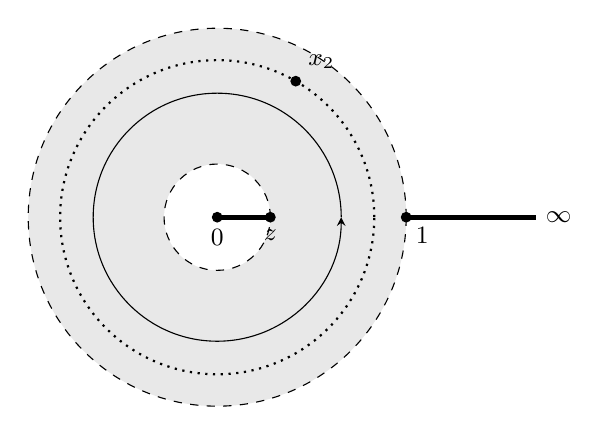
\begin{tikzpicture}[scale=1.5,>=stealth,every node/.style={font=\small}]
 \fill[gray!18] (0,0) circle (1.6);
 \fill[white] (0,0) circle (0.45);
 \draw[dashed] (0,0) circle (1.6);
 \draw[dashed] (0,0) circle (0.45);
 \draw[->] (1.05,0) arc (0:360:1.05);
 \draw[dotted,thick] (0,0) circle (1.33);
 \draw[line width=1.8pt] (0,0)--(0.45,0);
 \draw[line width=1.8pt] (1.6,0)--(2.7,0);
 \fill (0,0) circle (1.3pt) node[below=1pt] {\(0\)};
 \fill (0.45,0) circle (1.3pt) node[below=1pt] {\(z\)};
 \fill (1.6,0) circle (1.3pt) node[below right] {\(1\)};
 \fill (60:1.33) circle (1.3pt) node[above right=1pt] {\(x_2\)};
 \node[right] at (2.7,0) {\(\infty\)};
\end{tikzpicture}
\caption{The \(x\)-plane of Lemmas~\ref{lem:saddle} and~\ref{lem:bergman-det},
drawn for \(0<z<1\).  The curve \(Y^2=x(x-z)(x-1)\) is branched at \(0\),
\(z\), \(1\) and \(\infty\); thick segments show the cuts.  The dashed circles
are \(|x|=|z|\) and \(|x|=1\); the Laurent expansion of \(\Omega(x;z)\) in
Lemma~\ref{lem:saddle}(iii) is taken on the shaded annulus between them.  For
fixed \(x_2\), the dotted circle \(|x_1|=|x_2|\) separates the inner and outer
patches of Step~2 of Lemma~\ref{lem:bergman-det}, and Step~3 sums the residues
of \(\frac x2W_{\mathrm{no}}(x,x)\) at \(x=0\) and \(x=z\) inside the oriented
circle \(|x|=r\).}
\label{fig:x-plane}
\end{figure}

\begin{lemma}[Diagonalization and the Wiener--Hopf saddle point]
\label{lem:saddle}
\begin{enumerate}\setlength{\itemsep}{1pt}\setlength{\topsep}{3pt}
\item[(i)] The generating functions \(A\) and \(B\) of~\eqref{eq:AB-gf}
  solve the order-\(\omega^0\) part of~\eqref{eq:S-pde}.  For every \(k\geq1\) they satisfy
  \(-\frac12\sum_{n=1}^{k-1}B_{n,k-n}=\frac{k-1}{16}\).
\item[(ii)] Setting \(p(w)=4w/(1+w)^2\),
  \(t_n(\sigma):=[w^{-n}]\sum_{m=1}^\infty\sigma_m p(w)^{-m}\), and
  \(g(w):=2i\sum_{n=1}^\infty n t_n w^n\), one has
  \(S^{(0)}(\sigma)=-4i\sum_{n=1}^\infty(-1)^{n-1}t_n-2\sum_{n=1}^\infty n t_n^2\).
\item[(iii)] Write
  \begin{align*}
   \Omega(x;z)&:=\Bigl({}_2F_1(\tfrac12,\tfrac12;1;z)\sqrt{1-x}\sqrt{1-z/x}\Bigr)^{-1}\\
   &=1+\sum_{m=1}^\infty a_m(z)x^m+\sum_{m=1}^\infty a_m(z)(z/x)^m,
  \end{align*}
  the Laurent expansion on \(|z|<|x|<1\).  The exact saddle point is
  \(\sigma_{*,m}(z)=i\frac{a_m(z)}{m}z^m\) (\(m\geq1\)).  With \(g_*\) and
  \(t_{*,n}\) the values of \(g\) and \(t_n\) at \(\sigma=\sigma_*\),
  \begin{equation}\label{eq:saddle-values}
   \mathcal I_0(z)=\log\frac{16q(z)}{z},\qquad
   1-g_*(1)=\theta_4(q(z))^{-2},\qquad
   1-g_*(-1)=\theta_3(q(z))^{-2}.
  \end{equation}
\end{enumerate}
\end{lemma}

\begin{proof}
(i) Set \(s_1=\sqrt{1-p}\), \(s_2=\sqrt{1-y}\) and \(s_3=\sqrt{1-x}\).
Substituting~\eqref{eq:AB-gf}, the \(\sigma^0\), \(\sigma^1\) and \(\sigma^2\)
components of the order-\(\omega^0\) PDE become the following identities of
rational functions in \((s_1,s_2,s_3)\):
\begin{align*}
 iA(p)-\tfrac14 A(p)^2-\frac{p}{1-p}&=0,\\
 (2i-A(p))B(p,y)+y\partial_y\Bigl(\frac{pA(y)-yA(p)}{y-p}-\frac{p}{1-p}A(y)\Bigr)&=0,\\
 y\partial_y\Bigl(\frac{pB(y,x)-yB(p,x)}{y-p}-\frac{p}{1-p}B(y,x)\Bigr)\qquad\qquad&\\
 +x\partial_x\Bigl(\frac{pB(y,x)-xB(p,y)}{x-p}-\frac{p}{1-p}B(y,x)\Bigr)
 -B(p,y)B(p,x)&=0.
\end{align*}
On the diagonal, \(-\frac12 B(p,p)=\frac{p^2}{16(1-p)^2}
=\sum_{k=2}^\infty\frac{k-1}{16}p^k\).

(ii) Under \(p=p(w)=\frac{4w}{(1+w)^2}\) (\(|w|<1\)), we have
\(\sqrt{1-p}=\frac{1-w}{1+w}\) and \(\frac{dp}{p}=\frac{1-w}{1+w}\frac{dw}{w}\),
so \(\frac{1-w}{1+w}A(p(w))=-\frac{4iw}{1+w}=-4i\sum_{n\geq1}(-1)^{n-1}w^n\)
and
\[
 \frac{1-w}{1+w}\frac{1-v}{1+v}B\bigl(p(w),p(v)\bigr)
 =-\frac{2wv}{(1-wv)^2}
 =-2\sum_{n=1}^\infty n(wv)^n.
\]
Changing variables in \(\sum A_m\sigma_m=\oint\frac{dp}{2\pi i p}A(p)\sum\sigma_m p^{-m}\)
and in the double contour integral
\(\sum B_{m,n}\sigma_m\sigma_n=\oint\oint\frac{dp}{2\pi i p}\frac{dy}{2\pi i y}B(p,y)\sum\sigma_m p^{-m}\sum\sigma_n y^{-n}\)
gives (ii).

(iii) Put \(\Omega_+(x)=1+\sum_{m\geq1}a_m(z)x^m\),
\(\Omega_-(x)=1+\sum_{m\geq1}a_m(z)(z/x)^m\),
\(\sigma_{*,m}=i\frac{a_m(z)}{m}z^m\), and
\(f_*(x)=\sum_{m\geq1}\sigma_{*,m}x^{-m}\).
Then \(p\partial_p f_*(p)=-i(\Omega_-(p)-1)\), hence
\[
 w\partial_w f_*\bigl(p(w)\bigr)
 =-i\frac{1-w}{1+w}\bigl(\Omega_-(p(w))-1\bigr).
\]
Since \(p(w)=p(w^{-1})\), the function \(f_*(p(w))\) is invariant under
\(w\leftrightarrow w^{-1}\); its \(w^{-n}\) coefficient is \(t_{*,n}\), so
\(\frac{1-w}{1+w}(\Omega_-(p(w))-1)=i\sum_{n=1}^\infty n t_{*,n}(w^n-w^{-n})\).
The function
\[
 \Xi(w):=\frac{1-w}{1+w}\Omega(p(w);z)
 =\Bigl({}_2F_1\!\left(\tfrac12,\tfrac12;1;z\right)\sqrt{1-z/p(w)}\Bigr)^{-1}
\]
is invariant under \(w\leftrightarrow w^{-1}\) for the same reason.  Write
\(\frac{1-w}{1+w}\Omega_+(p(w))=1+\sum_{n=1}^\infty c_n w^n\).  Equating
\([w^{-n}]\Xi(w)=[w^n]\Xi(w)\) for \(n\geq1\) gives \(-int_{*,n}=c_n+int_{*,n}\), so \(c_n=-2int_{*,n}\) and
\begin{equation}\label{eq:wh-identity}
 \frac{1-w}{1+w}\Omega_+(p(w))=1-g_*(w).
\end{equation}
From (ii),
\(\partial_{\sigma_m}S^{(0)}(\sigma_*)=\oint\frac{dw}{2\pi i w}p(w)^{-m}(-\frac{4iw}{1+w}+2ig_*(w))\).
Substituting \(g_*(w)=1-\frac{1-w}{1+w}\Omega_+(p(w))\) simplifies the
parenthesis to \(2i\frac{1-w}{1+w}(1-\Omega_+(p(w)))\), so changing back to
\(p=p(w)\) gives
\[
 \partial_{\sigma_m}S^{(0)}(\sigma_*)
 =2i\oint\frac{dp}{2\pi i p}p^{-m}\bigl(1-\Omega_+(p)\bigr)
 =-2ia_m(z)
 =-2mz^{-m}\sigma_{*,m}
 =2mz^{-m}\bar\sigma_{*,m},
\]
verifying the saddle-point equations.

By stationarity at \((\sigma_*,\bar\sigma_*)\) and~\eqref{eq:jacobi-2},
\begin{align*}
 z\frac{d}{dz}\mathcal I_0(z)
 &=2\sum_{m=1}^\infty m^2 z^{-m}\sigma_{*,m}\bar\sigma_{*,m}
  =2\sum_{m=1}^\infty a_m(z)^2 z^m\\
 &=[x^0]\bigl(\Omega(x;z)^2\bigr)-1
  =\frac{1}{(1-z)\theta_3(q(z))^4}-1
  =z\frac{d}{dz}\log\frac{16q(z)}{z},
\end{align*}
and \(\mathcal I_0(0)=0\) gives \(\mathcal I_0(z)=\log(16q(z)/z)\).
For sufficiently small \(|z|\), \(z/p(w)=z(1+w)^2/(4w)\) is uniformly small on
a fixed annulus straddling \(|w|=1\).  Hence \(f_*(p(w))\) and the symmetric
function \(\Xi(w)\) extend holomorphically to that annulus, with exponentially
decaying Laurent coefficients, and the continued Wiener--Hopf identity
\[
 \Xi(w)=1-g_*(w)+i\sum_{n=1}^\infty nt_{*,n}(w^n-w^{-n})
\]
holds there.  At \(w=1\) (\(p(1)=1\)) and \(w=-1\) (\(p(-1)=\infty\)) the
terms \(w^n-w^{-n}\) vanish, and~\eqref{eq:jacobi-1} gives
\(1-g_*(1)=\Xi(1)=\theta_4^{-2}\) and \(1-g_*(-1)=\Xi(-1)=\theta_3^{-2}\).
\end{proof}

\begin{lemma}[Evaluation of the Gaussian determinant]
\label{lem:bergman-det}
As formal power series in \(z\),
\[
 \det\bigl(I-M(z)^2\bigr)^{-1/2}
 =(1-z)^{-1/8}\,{}_2F_1\!\left(\tfrac12,\tfrac12;1;z\right)^{-1/2}
 =(1-z)^{-1/8}\theta_3\bigl(q(z)\bigr)^{-1}.
\]
\end{lemma}

\begin{proof}
The proof assembles the Gaussian covariance into a kernel \(W(x_1,x_2)\).
Steps~1 and~2 show that, coefficientwise in \(z\), \(Y(x_1)W(x_1,x_2)\)
continues to a meromorphic function of \(x_1\) on \(\mathbb P^1\) whose only
pole is at \(x_1=x_2\), with principal part
\(Y(x_2)/(x_1-x_2)^2+Y'(x_2)/(x_1-x_2)\); with the symmetry of \(W\),
Liouville's theorem then determines \(W\) up to one series \(C(z)\).  Step~3
fixes \(C(z)\) by a zero-mode condition and obtains \(z\) times the
logarithmic derivative of the determinant as the sum of the residues of
\(\frac x2W_{\mathrm{no}}(x,x)\) at \(x=0\) and \(x=z\)
(Figure~\ref{fig:x-plane}).  The first paragraph and the bounds in
Steps~1 and~2 make every series converge coefficientwise in \(z\), so that
these arguments apply.

Set \(D=\mathrm{diag}(1,2,\dots)\), \(B^{(z)}_{m,n}=z^{m+n}B_{m,n}\),
\(M_1=D^{-1}B^{(z)}\) and \(M_2=D^{-1}B\), and form the formal Neumann series
\(K_{12}:=\sum_{r\geq0}(M_1M_2)^r\) and \(K_{21}:=\sum_{r\geq0}(M_2M_1)^r\) in
\(M_\infty(\mathbb Q[[z]])\); we work coefficientwise in \(z\).  Since
\((M_1)_{m,n}=O(z^{m+n})\), every coefficient \([z^j]M_1\) (\(j\geq1\)) is
supported on \(m+n\leq j\).  Hence for every \(j\geq1\), \([z^j]K_{12}\) has
finite row support, and \([z^j]K_{21}\) has finite column support, each column
being a finite linear combination of columns of \(M_2\).  The function
\(B(p,y)\) is holomorphic on \(\{|p|<1,|y|<1\}\), where
\(\operatorname{Re}\sqrt{1-p}>0\), so Cauchy's inequality gives
\(|B_{m,n}|\leq C_\rho\rho^{-m-n}\) for every \(0<\rho<1\).  The formal series
\(\det(I-M(z)^2)^{-1/2}=\exp(\frac12\sum_{k\geq1}\frac1k\Tr(M(z)^{2k}))\) is
therefore well defined coefficientwise.  Let \(\widetilde M(z)_{m,n}=z^{(m+n)/2}B_{m,n}/\sqrt{mn}\) be the
symmetrized matrix.  For sufficiently small \(|z|\) the formal series equals
\(\det_F(I-\widetilde M(z)^2)^{-1/2}\), with the branch equal to \(1\) at
\(z=0\), where \(\det_F\) is the trace-class Fredholm determinant.  Indeed,
with \(s_m=z^{m/2}m^{-1/2}\) one has
\(M(z)_{m,n}=s_m\widetilde M(z)_{m,n}s_n^{-1}\), so in every cyclic product
\(M(z)_{m_1m_2}M(z)_{m_2m_3}\cdots M(z)_{m_{2k}m_1}\) the factors \(s_{m_i}\)
cancel, and \(\Tr M(z)^{2k}=\Tr\widetilde M(z)^{2k}\) coefficientwise in
\(z\); each coefficient involves only finitely many cycles, since a cycle
has \(z\)-order \(m_1+\dots+m_{2k}\).  (The diagonal matrix
\(\mathrm{diag}(s_m)^{-1}\) is unbounded on \(\ell^2\) for \(0<|z|<1\), so the
similarity is used only in this termwise form.)  For small \(|z|\) the
entries of \(\widetilde M(z)\) are bounded by \(C_\rho(|z|^{1/2}/\rho)^{m+n}\).
Their absolute sum is then bounded by a geometric double series that tends to
\(0\) with \(z\), so \(\widetilde M(z)\) is trace class with trace norm less
than \(1\), and
\(\log\det_F(I-\widetilde M(z)^2)=-\sum_{k\geq1}\frac1k\Tr\widetilde M(z)^{2k}\)
is analytic in \(z\) and vanishes at \(z=0\).

Fix \(x_2\) with \(0<|x_2|<1\), and define the formal power series in \(z\),
\(W(x_1,x_2):=\frac{1}{(x_1-x_2)^2}+W_{\mathrm{no}}(x_1,x_2)\), where
\begin{multline*}
 W_{\mathrm{no}}(x_1,x_2)
 :=\sum_{m,n\geq1}\Bigl(A_{++,mn}x_1^{-m-1}x_2^{-n-1}+A_{--,mn}x_1^{m-1}x_2^{n-1}\\
  +A_{-+,mn}x_1^{m-1}x_2^{-n-1}+A_{+-,mn}x_1^{-m-1}x_2^{n-1}\Bigr)
\end{multline*}
with blocks \(A_{++}=-B^{(z)}K_{21}\), \(A_{--}=-BK_{12}\),
\(A_{-+}=BK_{12}M_1\), and \(A_{+-}=A_{-+}^T=B^{(z)}K_{21}M_2\).  Each
coefficient \([z^j]W_{\mathrm{no}}(x_1,x_2)\) converges locally normally on
\(\{0<|x_1|,|x_2|<1\}\): the coefficients \([z^r]M_1\) have finite row and
column support, and the Cauchy bound \(|B_{m,n}|\leq C_\rho\rho^{-m-n}\) holds
with \(\rho\in(\max(|x_1|,|x_2|),1)\).

\emph{Step 1 (Rational twist identity and polynomial growth).}  With
\(s_1=\sqrt{1-p}\) and \(s_2=\sqrt{1-y}\) (\(p-y=s_2^2-s_1^2\)),
\begin{align*}
 \sqrt{1-p}\left(B(p,y)-\frac{py}{(p-y)^2}\right)
 &=-py\left(\frac{1}{2s_2(s_1+s_2)^2}+\frac{s_1}{(s_2^2-s_1^2)^2}\right)\\
 &=-\frac{py(2-p-y)}{2\sqrt{1-y}\,(p-y)^2}.
\end{align*}
Set \(p=1/X\) (\(|Xy|<1\)) and define
\(f_n(X):=\sum_{m=1}^\infty B_{m,n}X^{-m-1}-nX^{n-1}\) for \(n\geq1\).  Then
\(P_n(X):=\sqrt{X(X-1)}\,f_n(X)\) is a polynomial of degree \(n\), namely
\[
 P_n(X)=-\frac12[y^{n-1}]\frac{(2X-1)-Xy}{(1-y)^{1/2}(1-Xy)^2}.
\]
Expanding \((1-y)^{-1/2}\) and \((1-Xy)^{-2}\) gives
\(|[X^{n-k}]P_n(X)|=O(\mathrm{poly}(n))\) uniformly in \(0\leq k\leq n\).
Hence \(|P_n(X)|\leq C_K\,\mathrm{poly}(n)\max(1,|X|)^n\) on every compact
\(X\)-set \(K\).

\emph{Step 2 (Coefficientwise meromorphic continuation and Liouville's theorem).}
Fix \(0<|x_2|<1\) and use \(D+BK_{12}M_1=DK_{21}\) and \(BK_{12}=DK_{21}M_2\):
\begin{itemize}\setlength{\itemsep}{1pt}
\item \emph{Inner patch (\(|x_1|<|x_2|\)):} expanding
  \((x_1-x_2)^{-2}=\sum_{m\geq1}mx_1^{m-1}x_2^{-m-1}\) and setting
  \(v(x_2):=K_{21}(x_2^{-\bullet-1}-M_2x_2^{\bullet-1})\) gives
  \(W(x_1,x_2)=-\sum_{n\geq1}v_n(x_2)z^{n-1}f_n(x_1/z)\), so
  \(\sqrt{x_1(x_1-z)}\,W(x_1,x_2)=-\sum_{n\geq1}v_n(x_2)z^nP_n(x_1/z)\).
  For each \(j\geq0\), \([z^j]v_n(x_2)\) is a finite linear combination of
  columns of \(M_2\), plus, for \(j=0\), the source
  \(x_2^{-n-1}-(M_2x_2^{\bullet-1})_n\).  A Cauchy radius
  \(|x_2|<\rho<1\) bounds these columns and \((M_2x_2^{\bullet-1})_n\) by
  \(O(\rho^{-n})\), so \(|[z^j]v_n(x_2)|=O(|x_2|^{-n})\).  In
  \([z^j]\sum_{n\geq1}v_n z^n P_n(x_1/z)\), the only contributing monomials
  from \(z^nP_n(x_1/z)\) have powers \(x_1^{n-k}\) with \(0\leq k\leq j\) and
  coefficients \(O(\mathrm{poly}(n)|x_2|^{-n})\), giving normal convergence
  on every compact disc \(|x_1|\leq r<|x_2|\).
\item \emph{Outer patch (\(|x_1|>|x_2|\), including \(\infty\)):} define
  \(w(x_2):=K_{12}(x_2^{\bullet-1}-M_1x_2^{-\bullet-1})\).  Expanding
  \((x_1-x_2)^{-2}=\sum_{m\geq1}mx_1^{-m-1}x_2^{m-1}\) gives
  \begin{align*}
   W(x_1,x_2)&=-x_1^{-2}\sum_{n\geq1}w_n(x_2)f_n(1/x_1),\\
   x_1\sqrt{x_1-1}\,W(x_1,x_2)&=i\sum_{n\geq1}w_n(x_2)P_n(1/x_1).
  \end{align*}
  Since
  \([z^0]w_n=x_2^{n-1}\) while \([z^j]w\) has finite support for every
  \(j\geq1\), the polynomial bound on \(P_n\) gives normal convergence of each
  \([z^j]\)-coefficient on compact subsets of \(|x_1|>|x_2|\), including
  \(x_1=\infty\).
\end{itemize}
Put \(Y(x):=\sqrt{x(x-z)(x-1)}\), so that \(Y(x)\sim x^{3/2}\) at \(\infty\).
Multiply the inner patch by \(\sqrt{x_1-1}\), which is holomorphic on
\(|x_1|<1\), and the outer patch by \(\sqrt{1-z/x_1}\), coefficientwise in
\(z\), with consistent branch choice.  Then each coefficient
\([z^j](Y(x_1)W(x_1,x_2))\) extends to a single-valued meromorphic function on
\(\mathbb P^1\), holomorphic at \(\infty\).  Its only singularity is the pole at
\(x_1=x_2\), with the principal part of \([z^j](Y(x_1)/(x_1-x_2)^2)\).  The
symmetric
polynomial
\(S(x_1,x_2):=\frac12[x_1x_2(x_1+x_2)-2(1+z)x_1x_2+z(x_1+x_2)]\)
satisfies \(S(x,x)=Y(x)^2\), \(\partial_{x_1}S(x,x)=Y(x)Y'(x)\) and
\(\deg_{x_1}S=2\).  The symmetry \(W(x_1,x_2)=W(x_2,x_1)\) and Liouville's
theorem on \(\mathbb P^1\), applied coefficientwise in \(z\), force
\[
 W(x_1,x_2)=\frac{S(x_1,x_2)}{Y(x_1)Y(x_2)(x_1-x_2)^2}+\frac{2C(z)}{Y(x_1)Y(x_2)}
\]
for a unique formal power series \(C(z)\in\mathbb Q[[z]]\).

\emph{Step 3 (Zero-mode condition and Cauchy residue).}  Since
\([z^j]W(x_1,x_2)\) has no \(x_1^{-1}\) term on \(0<|x_1|<1\) and the
diagonal double pole \((x_1-x_2)^{-2}\) has zero residue,
\(\oint_{|x_1|=r}W(x_1,x_2)\frac{dx_1}{2\pi i}=0\) coefficientwise in \(z\)
for \(0<r<1\) with \(r\neq|x_2|\).  As \(x_2\to\infty\), the coefficient of
\(x_2^{-3/2}\) in this identity is
\(\oint_{|x_1|=r}(x_1/2+2C(z))Y(x_1)^{-1}\frac{dx_1}{2\pi i}=0\).  With
\begin{align*}
 E_0(z)&:=[x^0](1-z/x)^{-1/2}(1-x)^{-1/2}
  =\sum_{n\geq0}\tbinom{-1/2}{n}^2z^n={}_2F_1(\tfrac12,\tfrac12;1;z),\\
 E_1(z)&:=[x^{-1}](1-z/x)^{-1/2}(1-x)^{-1/2}
  =\sum_{n\geq0}\tbinom{-1/2}{n}^2\frac{n+1/2}{n+1}z^{n+1},
\end{align*}
this gives \(2C(z)=-\frac12 E_1(z)/E_0(z)\).  Because \([z^{n+1}]z(1-z)E_0'(z)=\frac{1}{4(n+1)}\binom{-1/2}{n}^2\), we
have \(E_1(z)=zE_0(z)-2z(1-z)E_0'(z)\) and
\(2C(z)=-\frac{z}{2}+z(1-z)E_0'(z)/E_0(z)\).

On \(0<|x|<1\), only the diagonal entries of \(A_{-+}\) and
\(A_{+-}\) contribute to \([x^{-2}]W_{\mathrm{no}}(x,x)\), so in
\(\mathbb Q[[z]]\),
\begin{align*}
 \oint_{|x|=r}\frac{x}{2}W_{\mathrm{no}}(x,x)\frac{dx}{2\pi i}
 &=\Tr(BK_{12}M_1)
  =\Tr\bigl(DM(z)^2(I-M(z)^2)^{-1}\bigr)\\
 &=z\frac{d}{dz}\log\det\bigl(I-M(z)^2\bigr)^{-1/2}.
\end{align*}
Write \(P(x)=x(x-1)(x-z)\).  The polynomial identity
\(4P(x)(-2x+1+z)+P'(x)^2=(x^2-z)^2\) gives the coincidence limit
\[
 W_{\mathrm{no}}(x,x)=\lim_{x_1\to x}\bigl(W(x_1,x)-(x_1-x)^{-2}\bigr)
 =\frac{(x^2-z)^2}{8x^2(x-1)^2(x-z)^2}+\frac{2C(z)}{x(x-1)(x-z)}.
\]
For \(0<|z|<r<1\), sum the residues at \(x=0\) and \(x=z\), then expand at
\(z=0\):
\[
 \sum_{a\in\{0,z\}}\Res_{x=a}\!\left(\frac{x}{2}W_{\mathrm{no}}(x,x)\right)
 =\frac{z}{8(z-1)}+\frac{2C(z)}{2(z-1)}
 =\frac{z}{8(1-z)}-\frac12 z\frac{E_0'(z)}{E_0(z)}.
\]
Dividing by \(z\) and integrating gives
\(\det(I-M(z)^2)^{-1/2}=(1-z)^{-1/8}E_0(z)^{-1/2}\); the constant of
integration is fixed by the value \(1\) of both sides at \(z=0\).
By~\eqref{eq:jacobi-1}, \(E_0(z)^{1/2}=\theta_3(q(z))\).
\end{proof}

\subsection{External-weight and central-charge exponents}

\begin{lemma}[External-weight exponents]\label{lem:ext-exponents}
One has \(S^{(2)}_2(\sigma)=2\log(1-g(1))\) and
\(S^{(2)}_1(\sigma)=2\log(1-g(-1))\), and hence
\(\Phi_2(z)=-4\log\theta_4(q(z))\) and \(\Phi_1(z)=-4\log\theta_3(q(z))\).
\end{lemma}

\begin{proof}
Under \(p=p(w)=\frac{4w}{(1+w)^2}\) one has
\(\frac{dw}{w}=(1-p)^{-1/2}\frac{dp}{p}\), \(\frac{w}{(1+w)^2}=\frac{p}{4}\) and
\(\frac{w}{(1-w)^2}=\frac{p}{4}(1-p)^{-1}\).  Changing variables in the
contour representations
\[
 g(\pm1)=2i\oint\frac{dw}{2\pi i w}\frac{\pm w}{(1\mp w)^2}\sum_m\sigma_m p(w)^{-m}
\]
gives
\(g(1)=\sum_{m=1}^\infty c^+_m\sigma_m\) and
\(g(-1)=\sum_{m=1}^\infty c^-_m\sigma_m\) with generating functions
\(C_+(p)=\frac{i}{2}p(1-p)^{-3/2}\) and
\(C_-(p)=-\frac{i}{2}p(1-p)^{-1/2}\).

Since \(L_k^{(0)}\) is a derivation, the equations
\(L_k^{(0)}(2\log(1-g(1)))=k\) and \(L_k^{(0)}(2\log(1-g(-1)))=-1\) are
equivalent to \(L_k^{(0)}g(1)=-\frac{k}{2}(1-g(1))\) and
\(L_k^{(0)}g(-1)=\frac12(1-g(-1))\) for all \(k\geq1\).  Set
\(s_1=\sqrt{1-p}\) and \(s_2=\sqrt{1-y}\).
\begin{itemize}\setlength{\itemsep}{1pt}
\item The \(\sigma^0\)-part generating function is
  \((i-\frac12 A(p))C_\pm(p)=\frac{i}{s_1}C_\pm(p)\), which equals
  \(-\frac{p}{2(1-p)^2}=\sum_{k\geq1}(-\frac{k}{2})p^k\) for \(g(1)\) and
  \(+\frac{p}{2(1-p)}=\sum_{k\geq1}(+\frac12)p^k\) for \(g(-1)\).
\item The \(\sigma^1\)-part generating function is
  \(y\partial_y(\frac{pC_\pm(y)-yC_\pm(p)}{y-p}-\frac{p}{1-p}C_\pm(y))-B(p,y)C_\pm(p)\),
  which, as a rational function of \((s_1,s_2)\), equals
  \(+\frac{p}{2(1-p)^2}C_+(y)\) for \(g(1)\) and
  \(-\frac{p}{2(1-p)}C_-(y)\) for \(g(-1)\).
\end{itemize}
By uniqueness of \(S^{(2)}_1,S^{(2)}_2\) (Lemma~\ref{lem:lambda-expansion}),
\(S^{(2)}_2=2\log(1-g(1))\) and \(S^{(2)}_1=2\log(1-g(-1))\).  Evaluating
at \(\sigma_*\) via~\eqref{eq:saddle-values} yields \(\Phi_2=-4\log\theta_4\)
and \(\Phi_1=-4\log\theta_3\).
\end{proof}

\begin{lemma}[Central-charge exponent from two \(c=1\) Fock modules]\label{lem:central-charge}
One has
\[
 \exp\bigl(\Phi_c^{\mathrm{raw}}(z)-\mathcal I_0(z)\bigr)
 =\prod_{m=1}^\infty\bigl(1-q(z)^{2m}\bigr)^{12}
 =\frac{z}{16q(z)}(1-z)\theta_3\bigl(q(z)\bigr)^{12}.
\]
\end{lemma}

\begin{proof}
The series \(\Phi_c^{\mathrm{raw}}\) is defined through the solutions
\(S^{(1)}_c\) and \(S^{(2)}_c\) of the Ward hierarchy, which are not known in
closed form.  We obtain it by computing one quantity at \(c=2\) in two ways.
Step~1 decomposes the tensor product of two \(c=1\) Fock modules into \(c=2\)
Verma modules; the product of two Gaussian Ward solutions then becomes a sum of
\(c=2\) blocks with coefficients \(c_n(\omega^2)\).  Steps~2 and~3 compute the
limits of these coefficients as \(\omega\to\infty\).  Step~2 builds the
large-\(\omega\) primaries from states of the neutral boson by an operator
\(U(W)\), and in Step~3 the adjoint \(U(W)^\dagger\) acts on the boson current
as a conformal map, which makes the limit explicit.  Step~4 applies
Proposition~\ref{prop:gaussian-limit} at \(c=2\) to each block and solves for
\(\Phi_c^{\mathrm{raw}}\).

Consider the unitary tensor product
\(\mathcal H_\omega:=\mathcal F_{0,\omega}^{(1)}\otimes\mathcal F_{0,0}^{(2)}\)
of two \(c=1\) Fock modules.  The first has oscillators \(v_m\) and weight
\(\omega^2\), \(\omega>0\); the second has oscillators \(u_m\) and weight
\(0\).  The diagonal action \(L_k^{\mathrm{tot}}=l_k^{(1)}+l_k^{(2)}\) is a unitary
Virasoro action of central charge \(2\).

\emph{Step 1 (Exact \(c=2\) decomposition).}  At \(\eta=0\) and
\(\Delta_1=\Delta_2=\frac1{16}\), the pure Gaussians
\(F_1(v)=\exp(\omega\sum A_mv_m+\sum B_{m,n}v_mv_n)\) and
\(F_2(u)=\exp(\sum B_{m,n}u_mu_n)\) solve the exact finite-\(\omega\) Fock
Ward equations \(l_k^{(1)}F_1=(l_0^{(1)}+\frac{k-1}{16})F_1\) and
\(l_k^{(2)}F_2=(l_0^{(2)}+\frac{k-1}{16})F_2\).  This follows
from~\eqref{eq:AB-gf} and~\eqref{eq:S-pde} at \(\eta=0\), with the diagonal
value \(-\frac12\sum_{n=1}^{k-1}B_{n,k-n}=\frac{k-1}{16}\) of
Lemma~\ref{lem:saddle}(i).  Gaussian evaluation in the Fock spaces
(Proposition~\ref{prop:gaussian-limit} and Lemma~\ref{lem:saddle}(iii)) gives the
pairings below.  They are pairings in the Fock modules; the second one is
not a Verma block, since the Verma Gram matrix is singular at
\((c,\Delta)=(1,0)\):
\begin{align*}
 G_{\mathrm{charged}}(\omega;z)
 &:=\langle\widetilde F_1(\bar v),F_1(z^\bullet v)\rangle_{\mathcal F^{(1)}_{0,\omega}}
  =\det\bigl(I-M(z)^2\bigr)^{-1/2}\Bigl(\frac{16q(z)}{z}\Bigr)^{\omega^2},\\
 G_{\mathrm{neutral}}(z)
 &:=\langle\widetilde F_2(\bar u),F_2(z^\bullet u)\rangle_{\mathcal F^{(2)}_{0,0}}
  =\det\bigl(I-M(z)^2\bigr)^{-1/2}.
\end{align*}
The product \(F_{\mathrm{tot}}=F_1F_2\) solves the
exact \(c=2\), \(\Delta_1=\Delta_2=\frac18\) Ward equation
\(L_k^{\mathrm{tot}}F_{\mathrm{tot}}=(L_0^{\mathrm{tot}}+\frac{k-1}{8})F_{\mathrm{tot}}\).
At \(c=2\), every Kac weight is either nonpositive or nonreal, as in the
proof of Lemma~\ref{lem:fock-verma}(i), so every Verma module
\(M(2,\omega^2+n)\) (\(n\geq0\), \(\omega>0\)) is irreducible and unitary.
Hence \(\mathcal H_\omega\) decomposes orthogonally as
\(\mathcal H_\omega=\bigoplus_{n=0}^\infty\bigoplus_{j=1}^{p(n)}M_{2,\omega^2+n}^{(j)}\),
where \(M^{(j)}_{2,\omega^2+n}\) is the \(j\)-th copy of \(M(2,\omega^2+n)\).  The
multiplicities come from the graded characters in the grading variable \(t\),
\(\prod_{m\geq1}(1-t^m)^{-2}/\prod_{m\geq1}(1-t^m)^{-1}=\sum_{n\geq0}p(n)t^n\),
so the primary space
\(\mathcal P_n(\omega):=\{P\in(\mathcal H_\omega)_n:L_k^{\mathrm{tot}}P=0\ \forall k\geq1\}\)
has dimension \(p(n)\).  Because the Ward equations uniquely determine all
descendant projections of \(F_{\mathrm{tot}}\) inside each irreducible summand
\(M_{2,\omega^2+n}^{(j)}\) from its primary component, orthogonal projection
gives, in \(\mathbb C[[z]]\),
\begin{equation}\label{eq:c2-decomp}
 G_{\mathrm{charged}}(\omega;z)\,G_{\mathrm{neutral}}(z)
 =\sum_{n=0}^\infty c_n(\omega^2)\,z^n\,\mathcal B(2,\omega^2+n,\tfrac18;z),
\end{equation}
where
\(c_n(\omega^2)=\sum_{a,b}\overline{\langle P_a,F_1F_2\rangle}(G^{(n)}(\omega)^{-1})_{a,b}\langle P_b,F_1F_2\rangle\)
for any basis \(\{P_a\}\) of \(\mathcal P_n(\omega)\) with Gram matrix
\(G^{(n)}(\omega)_{a,b}=\langle P_a,P_b\rangle\); in~\eqref{eq:c2-decomp} the scalar
\(\tfrac18\) in the external slot means that all four external weights are
\(\tfrac18\).

\emph{Step 2 (Large-\(\omega\) primaries).}
Rescaling \(v_m=i\omega W_m\) gives
\[
 l_k^{(1)}=D_k+\frac{1}{4\omega^2}\sum_{r=1}^{k-1}\partial_{W_r}\partial_{W_{k-r}},
\]
where \(D_k:=\partial_{W_k}+\sum_{m\geq1}mW_m\partial_{W_{m+k}}\) is \(D_k(\infty)\) of
Lemma~\ref{lem:lambda-expansion} after \(\sigma_m=iW_m\).  Fix a
level \(n\geq0\).  On the finite-dimensional space \((\mathcal H_\omega)_n\),
consider the joint map given by the primary conditions
\(L_k^{\mathrm{tot}}P\) (\(1\leq k\leq n\)) and the evaluation
\(\operatorname{ev}_0(P):=P|_{W=0}\in(\mathcal F^{(2)}_{0,0})_n\).  At
\(\omega^{-2}=0\) this map is injective: a nonzero \(P\) in its kernel has
\(\operatorname{ev}_0P=0\), so its nonzero part of lowest positive \(W\)-level
lies in \(\bigcap_{k=1}^n\ker D_k\), contrary to the injectivity in the proof of
Lemma~\ref{lem:lambda-expansion}(i).  A full-rank minor therefore stays
nonzero for all sufficiently large \(\omega\).  Since
\(\dim\mathcal P_n(\omega)=p(n)=\dim(\mathcal F^{(2)}_{0,0})_n\), the
restriction
\(\operatorname{ev}_0|_{\mathcal P_n(\omega)}:\mathcal P_n(\omega)\to(\mathcal F^{(2)}_{0,0})_n\)
is a linear isomorphism for all sufficiently large \(\omega\) at each fixed
\(n\).  Its inverse \(w\mapsto P_w\) is regular in \(\omega^{-2}\) at
\(\omega^{-2}=0\), with \(P_w(i\omega W,u)=U(W)w(u)+O(\omega^{-2})\), where
\(U(W):\mathcal F^{(2)}\to\mathcal F^{(2)}[[W]]\) acts finitely on each
homogeneous component and uniquely solves \((D_k+l_k^{(2)})U(W)=0\)
(\(\forall k\geq1\)) with \(U(0)=\mathrm{id}\).

Since \(W_m=v_m/(i\omega)\), the part of \(P_w\) of charged degree \(k\) is
\(O(\omega^{-k})\), and parts of different charged degree are orthogonal, so
\(G^{(n)}(\omega)_{w_1,w_2}=\langle w_1,w_2\rangle_{\mathcal F^{(2)}}+O(\omega^{-2})\).
In the pairing \(\langle P_w,F_1F_2\rangle\), each monomial in
\(\overline{W_m}=i\bar v_m/\omega\) paired against the charged Gaussian
\(F_1(v)\) evaluates by Wick's theorem to the product of saddle means
\(W_{*,m}:=\frac{iA_m}{2m}=\frac{1}{m\cdot 4^m}\binom{2m}{m}\in\mathbb R\)
plus \(O(\omega^{-2})\) from quadratic contractions.  Take the adjoint of
\(U(W)\) level by level for real \(W\) and evaluate at \(W_*\).  Then
\[
 c_n^\infty:=\lim_{\omega\to\infty}c_n(\omega^2)
 =\bigl\|\bigl(U(W_*)^\dagger F_2\bigr)_n\bigr\|_{\mathcal F^{(2)}}^2.
\]

\emph{Step 3 (Exact diagonalization of \(U(W_*)^\dagger F_2\)).}  Taking
the adjoint of \(D_kU(W)=-l_k^{(2)}U(W)\) in real variables \(W\) yields
\(D_k(U(W)^\dagger)=-U(W)^\dagger l_{-k}^{(2)}\) with
\(U(0)^\dagger=\mathrm{id}\).  Define the free-boson current
\(\alpha(x):=\sum_{n\neq0}\alpha_n x^{-n-1}\) on \(\mathcal F^{(2)}\) by
\(\alpha_n=\frac{i}{\sqrt2}\partial_{u_n}\) and
\(\alpha_{-n}=-i\sqrt2\,n u_n\) (\(n\geq1\)), which satisfies
\([l_{-k}^{(2)},\alpha(x)]=\partial_x(x^{1-k}\alpha(x))\).  Then
\(\Psi(W,x):=U(W)^\dagger\alpha(x)(U(W)^\dagger)^{-1}\) satisfies
\(D_k\Psi=-\partial_x(x^{1-k}\Psi)\) with \(\Psi(0,x)=\alpha(x)\).  Differentiating
\(f(x;W):=x\exp(-\sum_{m\geq1}W_m x^{-m})\) gives
\(D_k(f(x;W))=-x^{1-k}f'(x;W)\), so \(f'(x;W)\alpha(f(x;W))\) solves the
same system with the same initial value.  The solution is unique, by
triangularity in the \(W\)-adic filtration and the joint injectivity of the
family \((D_k)\) on each positive \(W\)-level,
so \(U(W)^\dagger\alpha(x)(U(W)^\dagger)^{-1}=f'(x;W)\alpha(f(x;W))\) before
specialization.  In other words, \(U(W)^\dagger\) acts on the current as the
conformal map \(x\mapsto f(x;W)\).

At \(W=W_*\),
\[
 \sum_{m\geq1}\frac{1}{m\cdot 4^m}\binom{2m}{m}y^m
 =\int_0^y\frac{(1-t)^{-1/2}-1}{t}\,dt
 =\log\frac{4(1-\sqrt{1-y})}{y(1+\sqrt{1-y})},
\]
so \(X=f(x;W_*)\) has inverse \(x(X)=X+\frac12+\frac{1}{16X}\), with
\(\sqrt{x(X)(x(X)-1)}=X-\frac{1}{16X}\).  By Step~1 of
Lemma~\ref{lem:bergman-det}, \(\sqrt{x(x-1)}\alpha(x)F_2(u)\) has only
non-negative powers of \(x\), i.e.,
\(\oint x^{k-1}\sqrt{x(x-1)}\alpha(x)\,dx\cdot F_2=0\) for all \(k\geq1\).
Applying \(U(W_*)^\dagger\) and changing variables to \(X=f(x;W_*)\) gives
\[
 \oint x(X)^{k-1}\!\left(X-\frac{1}{16X}\right)\alpha(X)\,dX\cdot\bigl(U(W_*)^\dagger F_2\bigr)=0
 \qquad(\forall k\geq1).
\]
The function \(x(X)\) is invariant under \(X\mapsto\frac{1}{16X}\) and has
leading term \(X\), so, by triangularity, the Laurent polynomials
\(x(X)^{k-1}(X-\frac{1}{16X})\) (\(k\geq1\)) span the same space as the
Laurent polynomials \(X^m-16^{-m}X^{-m}\), \(m\geq1\).  Hence
\((\alpha_m-16^{-m}\alpha_{-m})(U(W_*)^\dagger F_2)=0\) for every \(m\geq1\).
In the variables \(u_m\) this reads
\(\partial_{u_m}(U(W_*)^\dagger F_2)=-\frac{2m}{16^m}u_m(U(W_*)^\dagger F_2)\).  Because \(l_{-k}^{(2)}\) strictly raises level,
\((U(W_*)^\dagger F_2)_0=F_2(0)=1\), and therefore
\[
 U(W_*)^\dagger F_2(u)=\exp\!\left(-\sum_{m=1}^\infty\frac{m}{16^m}u_m^2\right).
\]
Computing its level-\(n\) Fock norm squared from~\eqref{eq:fock-ip} gives
\begin{align*}
 \sum_{n=0}^\infty 16^n c_n^\infty q^n
 &=\prod_{m=1}^\infty\sum_{k=0}^\infty\frac{m^{2k}(2k)!}{(k!)^2(2m)^{2k}}q^{2mk}\\
 &=\prod_{m=1}^\infty\sum_{k=0}^\infty\binom{-1/2}{k}(-q^{2m})^k
  =\prod_{m=1}^\infty(1-q^{2m})^{-1/2}.
\end{align*}

\emph{Step 4 (Matching~\eqref{eq:c2-decomp}).}  Divide~\eqref{eq:c2-decomp}
by \((16q/z)^{\omega^2}\) and take the limit \(\omega\to\infty\)
coefficientwise; at order \(z^N\) the sum has \(0\leq n\leq N\).  By
Lemma~\ref{lem:lambda-expansion}, Proposition~\ref{prop:gaussian-limit} and Lemmas~\ref{lem:saddle}--\ref{lem:ext-exponents}, at \(c=2\)
(\(\eta^2=\frac{1}{24}\), \(\Delta_j-\frac{1}{16}=\frac{1}{16}\)):
\begin{itemize}\setlength{\itemsep}{1pt}
\item the left-hand side tends to
  \(((1-z)^{-1/8}\theta_3^{-1})^2=(1-z)^{-1/4}\theta_3^{-2}\);
\item on the right-hand side, each term \(\mathcal B(2,\omega^2+n,\tfrac18;z)\)
  has \(\Delta-\eta^2=\omega^2+n-\frac{1}{24}\), so its exponential factor
  combines with \(z^n\) to give \((16q)^n(16q/z)^{-1/24}\); summing over \(n\)
  yields
  \[
   \Bigl(\prod_{m=1}^\infty(1-q^{2m})^{-1/2}\Bigr)
   \Bigl(\frac{16q}{z}\Bigr)^{-1/24}(1-z)^{-1/8}\theta_3^{-1}
   \exp\Bigl(\frac{1}{24}\Phi_c^{\mathrm{raw}}+\frac18(\Phi_1+\Phi_2)\Bigr).
  \]
\end{itemize}
Since \(\frac18(\Phi_1+\Phi_2)=-\frac12\log(\theta_3\theta_4)=-\frac18\log(1-z)-\log\theta_3\),
the factor \((1-z)^{-1/4}\theta_3^{-2}\) cancels on both sides, leaving
\(\exp(\frac{1}{24}(\Phi_c^{\mathrm{raw}}-\mathcal I_0))=\prod_{m\geq1}(1-q^{2m})^{1/2}\).
Taking the \(24\)th power and using~\eqref{eq:jacobi-3} proves the two
expressions.
\end{proof}

\begin{proof}[Proof of Theorem~\ref{thm:large-delta}]
Let \(\eta>0\), so that \(c=1+24\eta^2>1\), and let
\(\Delta_1,\dots,\Delta_4\in\mathbb R\).  Combining
Lemma~\ref{lem:lambda-expansion},
Proposition~\ref{prop:gaussian-limit} and
Lemmas~\ref{lem:saddle}--\ref{lem:central-charge} with
\(\Delta=\omega^2+\eta^2\) and \(\theta_4^4=(1-z)\theta_3^4\) gives, in
\(\mathbb C[[z]]\),
\begin{align*}
 \lim_{\Delta\to\infty}\Bigl(\frac{16q}{z}\Bigr)^{-\Delta}\mathcal B(c,\Delta,\Delta_i;z)
 &=(1-z)^{-1/8}\theta_3^{-1}
  \Bigl(\frac{z}{16q}(1-z)\theta_3^{12}\Bigr)^{\frac{c-1}{24}}\\
 &\qquad\times\theta_3^{-4(\Delta_1+\Delta_4-\frac18)}
  \theta_4^{-4(\Delta_2+\Delta_3-\frac18)}\\
 &=\Bigl(\frac{16q}{z}\Bigr)^{-\frac{c-1}{24}}
  (1-z)^{\frac{c-1}{24}-\Delta_2-\Delta_3}
  \theta_3^{\frac{c-1}{2}-4(\Delta_1+\Delta_2+\Delta_3+\Delta_4)}\\
 &=\Bigl(\frac{16q}{z}\Bigr)^{-\Delta}\widetilde\Phi(c,\Delta,\Delta_i;q(z)).
\end{align*}
Divide by the \(\Delta\)-independent last expression and use
\(\mathcal B=\widetilde\Phi H\) from~\eqref{eq:H-def}.  This gives
\(\lim_{\Delta\to\infty}H_N=\delta_{N,0}\) for every \(N\geq0\), and
Lemma~\ref{lem:fock-verma}(iii) extends the limit to all
\((c,\Delta_1,\dots,\Delta_4)\in\mathbb C^5\).
\end{proof}

\begin{remark*}[The semiclassical picture and the case \(c=1\)]
Proposition~\ref{prop:gaussian-limit} is a semiclassical expansion with
\(\omega^2\) in the role of \(1/\hbar\): \(\mathcal I_0\) is the value of the
action at the saddle point, \(\det(I-M(z)^2)^{-1/2}\) is the one-loop factor,
and \(\Phi_1\), \(\Phi_2\) and \(\Phi_c^{\mathrm{raw}}\) are the first
corrections.  Be\c{s}ken, Datta and Kraus work in the same oscillator
realization and obtain the leading factor
\((16q)^\Delta\)~\cite[\S4.3]{BeskenDattaKraus2019}.  At \(c=1\) and
\(\Delta_1=\dots=\Delta_4=\frac1{16}\), Step~1 of the proof of
Lemma~\ref{lem:central-charge} shows that the Gaussian \(F_1\) solves the Ward
equations exactly.  For real \(\Delta=\omega^2>0\) at which \(M(1,\Delta)\) is
irreducible, the argument of Lemma~\ref{lem:fock-verma}(ii) identifies the
pairing \(G_{\mathrm{charged}}\) with the cross-ratio series, so
\(\mathcal B=\widetilde\Phi\).  Both sides are rational in \(\Delta\)
coefficientwise in \(z\), so \(\mathcal B=\widetilde\Phi\) and \(H=1\) at every
\(\Delta\) at which \(M(1,\Delta)\) is irreducible.  This is Zamolodchikov's closed
form of the Ashkin--Teller block~\cite[(2.28)]{Zamolodchikov1986}; see
also~\cite[(2.13)]{IorgovLisovyyTykhyy2013}.
\end{remark*}

\appendix
\section{Finite sums in the Gaussian calculation}\label{app:gaussian}

This appendix gives the finiteness statements used in the proof of
Proposition~\ref{prop:gaussian-limit}, in the notation of that proof: \(N\geq0\)
is fixed, all computations take place in \(\mathbb C[[z]]/(z^{N+1})\),
\(D=\mathrm{diag}(1,\dots,N)\), \(M_1=D^{-1}B^{(z)}\) and \(M_2=D^{-1}B\).

The matrix
\(Q_0^{-1}(Q(z)-Q_0)=\bigl(\begin{smallmatrix}0&-M_2\\-M_1&0\end{smallmatrix}\bigr)\)
reduces modulo \(z\) to a strictly block upper-triangular matrix, and its square
\(\mathrm{diag}(M_2M_1,M_1M_2)\) is \(O(z^2)\).  Thus
\(Q_0^{-1}(Q(z)-Q_0)\) is nilpotent in \(M_{2N}(\mathbb C[[z]]/(z^{N+1}))\),
and the formal Gaussian determinant and covariance are finite algebraic sums.
The Neumann block inverse is
\[
 Q(z)^{-1}
 =\bigl(I+Q_0^{-1}(Q-Q_0)\bigr)^{-1}Q_0^{-1}
 =\frac12\begin{pmatrix}K_{21}M_2D^{-1}&K_{21}D^{-1}\\K_{12}D^{-1}&K_{12}M_1D^{-1}\end{pmatrix},
\]
with \(K_{21}=(I-M_2M_1)^{-1}\) and \(K_{12}=(I-M_1M_2)^{-1}\).

For the centered variables \((U,V)\) of the proof, the Neumann inverse gives
\begin{align*}
 \operatorname{Cov}(U_m,U_n)&=O(z^{m+n}),\qquad
 \operatorname{Cov}(V_m,V_n)=O(z^{m+n}),\\
 \operatorname{Cov}(U_m,V_n)&=\frac{\delta_{m,n}}{2m}z^m+O(z^{m+n}).
\end{align*}
Consequently, every Wick contraction of a pair of modes of weights \(m,n\) has
\(z\)-order at least \(\frac{m+n}{2}\), and every Wick monomial in \((U,V)\) of
total oscillator weight \(L\) has \(z\)-order at least \(\lceil L/2\rceil\).
Every saddle factor \(\sigma_{*,m},\bar\sigma_{*,m}\) has \(z\)-order at
least \(m\).  Modulo \(z^{N+1}\), finitely many modes contribute, and the
contributing Wick monomials have total oscillator weight at most \(2N\).  The
shifts and \(\omega^{-1}\)-extractions therefore take place in
\(\mathbb C[[z]]/(z^{N+1})\).

\section*{AI-use disclosure}

AI systems contributed substantially to developing and checking the
proofs, writing the verification scripts, and drafting and revising the
manuscript. The author directed the research and takes responsibility
for all mathematical claims, citations, computations and wording.

\section*{Code availability}

The script \path{sphere/tools/audit_large_delta.py} in
\href{https://github.com/skypher/virasoro}{github.com/skypher/virasoro}
checks Lemmas~\ref{lem:saddle}, \ref{lem:bergman-det}
and~\ref{lem:ext-exponents} in exact symbolic and rational arithmetic, the
first two through \(z^7\); it checks the change of variables used in Step~3
of the proof of Lemma~\ref{lem:central-charge} and the product
identity~\eqref{eq:jacobi-3} through \(q^{12}\), and the degree inequality of
Theorem~\ref{thm:large-delta} for \(N\leq5\) at three choices of
\((c,\Delta_1,\dots,\Delta_4)\).  The proofs use no computer calculation.

{\small
\begin{thebibliography}{GRSS22}
\setlength{\itemsep}{0pt plus 0.5pt}
\setlength{\parskip}{0pt}

\bibitem[AK26]{ArtemevKhromov2026}
A.~Artemev and D.~Khromov,
\emph{WKB asymptotics for multipoint Virasoro conformal blocks and applications},
Phys.\ Rev.\ D \textbf{114} (2026) 045002,
\href{https://doi.org/10.1103/9y4x-9b4p}{doi:\allowbreak 10.1103/9y4x-9b4p},
\href{https://arxiv.org/abs/2603.08194}{arXiv:2603.08194}.

\bibitem[BDK20]{BeskenDattaKraus2019}
M.~Be\c{s}ken, S.~Datta and P.~Kraus,
\emph{Semi-classical Virasoro blocks: proof of exponentiation},
JHEP \textbf{01} (2020) 109,
\href{https://doi.org/10.1007/JHEP01(2020)109}{doi:\allowbreak 10.1007/JHEP01(2020)109},
\href{https://arxiv.org/abs/1910.04169}{arXiv:1910.04169}.

\bibitem[GRSS22]{GhosalRemySunSun2022}
P.~Ghosal, G.~R\'emy, X.~Sun and Y.~Sun,
\emph{Analyticity and symmetry of Virasoro conformal blocks via Liouville CFT},
preprint (1~November 2022),
\href{https://guillaumeremy92.github.io/files/Modular_Equation.pdf}%
{guillaumeremy92.github.io/\allowbreak files/\allowbreak Modular\_Equation.pdf}.

\bibitem[IK11]{IoharaKoga2011}
K.~Iohara and Y.~Koga,
\emph{Representation Theory of the Virasoro Algebra},
Springer Monographs in Mathematics, Springer (2011),
\href{https://doi.org/10.1007/978-0-85729-160-8}%
{doi:\allowbreak 10.1007/978-0-85729-160-8}.

\bibitem[ILT13]{IorgovLisovyyTykhyy2013}
N.~Iorgov, O.~Lisovyy and Yu.~Tykhyy,
\emph{Painlev\'e VI connection problem and monodromy of \(c=1\) conformal blocks},
JHEP \textbf{12} (2013) 029,
\href{https://doi.org/10.1007/JHEP12(2013)029}{doi:\allowbreak 10.1007/JHEP12(2013)029},
\href{https://arxiv.org/abs/1308.4092}{arXiv:1308.4092}.

\bibitem[Pol26b]{PolzerColliding2026}
L.~P.~Polzer,
\emph{Colliding poles of Virasoro conformal blocks at rational central
charge},
companion manuscript, version of November 25, 2026, in \href{https://github.com/skypher/virasoro}{github.com/skypher/virasoro}.

\bibitem[Rib26]{Ribault2026}
S.~Ribault,
\emph{Exactly solvable conformal field theories},
SciPost Phys.\ Lect.\ Notes \textbf{130} (2026),
\href{https://doi.org/10.21468/SciPostPhysLectNotes.130}%
{doi:\allowbreak 10.21468/SciPostPhysLectNotes.130},
\href{https://arxiv.org/abs/2411.17262v4}{arXiv:2411.17262v4}.

\bibitem[WW27]{WhittakerWatson1927}
E.~T.~Whittaker and G.~N.~Watson,
\emph{A Course of Modern Analysis}, 4th ed.,
Cambridge University Press (1927).

\bibitem[Zam84]{Zamolodchikov1984}
Al.~B.~Zamolodchikov,
\emph{Conformal symmetry in two dimensions: an explicit recurrence
formula for the conformal partial wave amplitude},
Commun.\ Math.\ Phys. \textbf{96} (1984) 419--422,
\href{https://doi.org/10.1007/BF01214585}{doi:\allowbreak 10.1007/BF01214585}.

\bibitem[Zam86]{Zamolodchikov1986}
Al.~B.~Zamolodchikov,
\emph{Two-dimensional conformal symmetry and critical four-spin correlation
functions in the Ashkin--Teller model},
Zh.\ Eksp.\ Teor.\ Fiz. \textbf{90} (1986) 1808--1818; English translation
in Sov.\ Phys.\ JETP \textbf{63} (1986) 1061.

\bibitem[Zam87]{Zamolodchikov1987}
Al.~B.~Zamolodchikov,
\emph{Conformal symmetry in two-dimensional space: recursion
representation of conformal block},
Theor.\ Math.\ Phys. \textbf{73} (1987) 1088--1093,
\href{https://doi.org/10.1007/BF01022967}{doi:\allowbreak 10.1007/BF01022967}.

\end{thebibliography}
}

\end{document}
